% Final thesis defense (PHANTOM)
% Build: cd paper/defense && pdflatex defense.tex && pdflatex defense.tex
\documentclass[aspectratio=169,11pt]{beamer}

\usepackage[utf8]{inputenc}
\usepackage[T1]{fontenc}
\usepackage{lmodern}
\usepackage{microtype}
\usepackage{amsmath,amssymb}
\usepackage{graphicx}
\usepackage{booktabs}
\usepackage{appendixnumberbeamer}
\usepackage{hyperref}
\usepackage{tikz}
\usetikzlibrary{arrows.meta,calc,positioning,fit,shapes.geometric,shapes.misc}

\graphicspath{{../src/chapters/figures/results/generated/final/plots/}{../src/chapters/}}

\usetheme[
  progressbar=frametitle,
]{moloch}
\molochset{sectionpage=none,subsectionpage=none}
\usefonttheme{professionalfonts}
\setbeamertemplate{frame numbering}[fraction]

% Palette
\definecolor{PhantomPaper}{HTML}{F6F1E9}
\definecolor{PhantomInk}{HTML}{0F1B2D}
\definecolor{PhantomSlate}{HTML}{24364C}
\definecolor{PhantomCyan}{HTML}{C97A3D}
\definecolor{PhantomIndigo}{HTML}{2F8F8A}

\setbeamercolor{normal text}{fg=PhantomSlate,bg=PhantomPaper}
\setbeamercolor{alerted text}{fg=PhantomCyan!95!black}
\setbeamercolor{example text}{fg=PhantomIndigo!95!black}
\setbeamercolor{palette primary}{fg=white,bg=PhantomInk}
\setbeamercolor{frametitle}{parent=palette primary}
\setbeamercolor{progress bar}{fg=PhantomCyan,bg=PhantomInk!28!white}
\setbeamercolor{title separator}{use=progress bar,parent=progress bar}
\setbeamercolor{structure}{fg=PhantomIndigo!90!black}
\setbeamercolor{block title}{fg=white,bg=PhantomIndigo!85!black}
\setbeamercolor{block body}{fg=PhantomSlate,bg=PhantomIndigo!8!white}
\setbeamercolor{alertblock title}{fg=white,bg=PhantomCyan!92!black}
\setbeamercolor{alertblock body}{fg=PhantomSlate,bg=PhantomCyan!10!white}
\setbeamercolor{exampleblock title}{fg=white,bg=PhantomIndigo!70!black}
\setbeamercolor{exampleblock body}{fg=PhantomSlate,bg=PhantomIndigo!8!white}

\setbeamertemplate{navigation symbols}{}
\setbeamertemplate{itemize item}{\small\raise0.3ex\hbox{$\bullet$}}
\setbeamertemplate{itemize subitem}{\tiny\raise0.2ex\hbox{$\circ$}}

\hypersetup{colorlinks=true,urlcolor=PhantomIndigo!90!black,linkcolor=PhantomSlate}

\title{PHANTOM}
\subtitle{Pricing Heuristics Against Non-human Transaction Orchestration Mechanisms}
\author{Daniel Rösel}
\institute{IE University, Madrid \\ Supervisor: Alberto Martín Izquierdo}
\date{\today}

\titlegraphic{%
  
\begin{tikzpicture}
    \shade[left color=PhantomCyan,right color=PhantomIndigo] (0,0) rectangle (0.55\paperwidth,0.06);
  \end{tikzpicture}%
}

\newcommand{\stagebar}[1]{}

\newcommand{\metriccard}[2]{%
  \begin{tikzpicture}
    \node[
      draw=PhantomInk,
      rounded corners=3pt,
      fill=PhantomCyan!10,
      minimum width=3.05cm,
      minimum height=1.25cm,
      align=center
    ] {\Large\bfseries #1\\[-0.2em]{\scriptsize #2}};
  \end{tikzpicture}%
}

\begin{document}

{
\setbeamercolor{background canvas}{bg=PhantomInk}
\begin{frame}[plain]
  \vfill
  \centering
  {\color{white}\Huge\bfseries PHANTOM\par}
  \vspace{0.6em}
  {\color{PhantomCyan}\rule{0.45\paperwidth}{0.06cm}\par}
  \vspace{0.8em}
  {\large\color{white!90!black}Pricing heuristics against non-human transaction orchestration\par}
  \vfill
  {\color{white!75!black}\normalsize Daniel Rösel\par}
  {\color{white!65!black}\small IE University \textbullet\ Supervisor: Alberto Martín Izquierdo\par}
  \vspace{1.2em}
  {\footnotesize\color{PhantomCyan!80!white}\href{https://velocitatem.github.io/PHANTOM/}{\texttt{velocitatem.github.io/PHANTOM}}}
  \vfill
\end{frame}
}

\begin{frame}{Roadmap: one argument in six stages (15 min)}
  \centering
  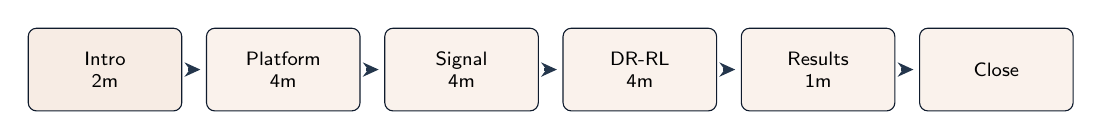
\begin{tikzpicture}[
    font=\scriptsize\sffamily,
    stage/.style={draw=PhantomInk,rounded corners=3pt,fill=PhantomCyan!10,minimum width=1.95cm,minimum height=1.05cm,align=center},
    flow/.style={-{Stealth[length=2.0mm,width=1.8mm]},line width=1pt,PhantomSlate}
  ]
    \node[stage,fill=PhantomCyan!14] (intro) {Intro\\2m};
    \node[stage,right=0.30cm of intro] (platform) {Platform\\4m};
    \node[stage,right=0.30cm of platform] (signal) {Signal\\4m};
    \node[stage,right=0.30cm of signal] (drrl) {DR-RL\\4m};
    \node[stage,right=0.30cm of drrl] (results) {Results\\1m};
    \node[stage,right=0.30cm of results] (close) {Close};

    \draw[flow,shorten <=2pt,shorten >=2pt] (intro.east) -- (platform.west);
    \draw[flow,shorten <=2pt,shorten >=2pt] (platform.east) -- (signal.west);
    \draw[flow,shorten <=2pt,shorten >=2pt] (signal.east) -- (drrl.west);
    \draw[flow,shorten <=2pt,shorten >=2pt] (drrl.east) -- (results.west);
    \draw[flow,shorten <=2pt,shorten >=2pt] (results.east) -- (close.west);
  \end{tikzpicture}

  \vspace{0.75em}
  \begin{block}{Main research question}
    How can dynamic pricing preserve margin integrity when transactions are increasingly mediated by non-human agents?
  \end{block}
  \vspace{0.35em}
  {\footnotesize Dynamic pricing has often been treated as a secondary optimization layer; agent-mediated shopping turns it into a primary margin-risk surface.}
  \stagebar{1}
\end{frame}

\begin{frame}{Agentic recon creates direct financial pressure on pricing power}
  \centering
  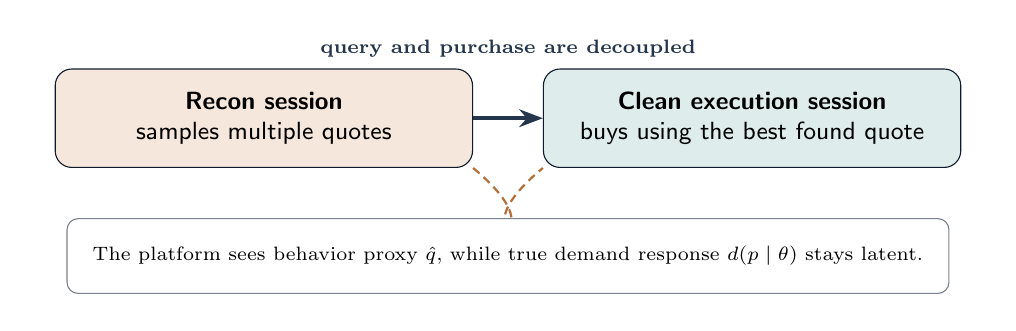
\begin{tikzpicture}[
    font=\small\sffamily,
    flow/.style={draw=PhantomInk,rounded corners=6pt,minimum width=5.3cm,minimum height=1.25cm,align=center},
    note/.style={draw=PhantomInk!55,rounded corners=4pt,minimum width=11.2cm,minimum height=0.95cm,align=center,fill=white,font=\scriptsize}
  ]
    \path[use as bounding box] (-6.1,-1.25) rectangle (6.1,2.25);
    \node<1->[flow,fill=PhantomCyan!18] (recon) at (-3.1,1.1)
      {\textbf{Recon session}\\samples multiple quotes};
    \node<2->[flow,fill=PhantomIndigo!16] (buy) at (3.1,1.1)
      {\textbf{Clean execution session}\\buys using the best found quote};
    \draw<2->[-{Stealth[length=3mm]},ultra thick,PhantomSlate] (recon.east) -- (buy.west);
    \node<2->[font=\scriptsize\bfseries,text=PhantomSlate] at (0,1.98)
      {query and purchase are decoupled};
    \draw<3->[densely dashed,thick,PhantomCyan!90!black]
      (recon.south east) .. controls +(1.15,-0.95) and +(-1.15,-0.95) .. (buy.south west);
    \node<3->[note] at (0,-0.65)
      {The platform sees behavior proxy $\hat q$, while true demand response $d(p\mid\theta)$ stays latent.};
  \end{tikzpicture}

  \vspace{0.25em}
  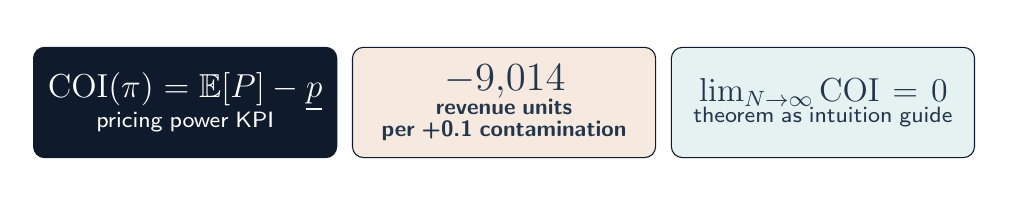
\begin{tikzpicture}[font=\scriptsize\sffamily,
    card/.style={draw=PhantomInk,rounded corners=4pt,minimum width=3.85cm,text width=3.55cm,minimum height=1.4cm,align=center}]
    \path[use as bounding box] (-6.05,-0.95) rectangle (6.05,0.95);
    \node<4->[card,fill=PhantomInk,text=white] at (-4.05,0)
      {\large$\mathrm{COI}(\pi)=\mathbb{E}[P]-\underline p$\\[-0.05em]\footnotesize pricing power KPI};
    \node<5->[card,fill=PhantomCyan!16,text=PhantomSlate] at (0,0)
      {\Large\bfseries$-9{,}014$\\[-0.05em]\footnotesize revenue units\\per +0.1 contamination};
    \node<6->[card,fill=PhantomIndigo!12,text=PhantomSlate] at (4.05,0)
      {\large$\lim_{N\to\infty}\mathrm{COI}=0$\\[-0.05em]\footnotesize theorem as intuition guide};
  \end{tikzpicture}

  \vspace{0.15em}
  \uncover<6->{\scriptsize\textit{The theorem is used to guide intuition: independent reconnaissance pressure can drive realizable prices toward the floor.}}\\[0.2em]
  \uncover<7->{\footnotesize\textbf{Implication:} most production dynamic pricing stacks are not yet ready for AI-agent traffic; when quote discovery and purchase split, session-based pricing overestimates willingness to pay.}
  \stagebar{1}
\end{frame}

\begin{frame}{The thesis answers one chain: mechanism \(\to\) signal \(\to\) control}
  \begin{enumerate}[<+->]\setlength{\itemsep}{0.45em}
    \item Can agent and human sessions be reliably distinguished from behavioral interaction signals alone?
    \item How do agents affect prices and revenue that can be generated?
    \item Can we make new policies that maintain margin in agent contaminated systems?
  \end{enumerate}

  \vspace{0.35em}
  \stagebar{1}
\end{frame}

\section{Platform Development}

\begin{frame}{Stage 1: We built a dual-loop platform to observe behavior and price exposure together}
  \centering
  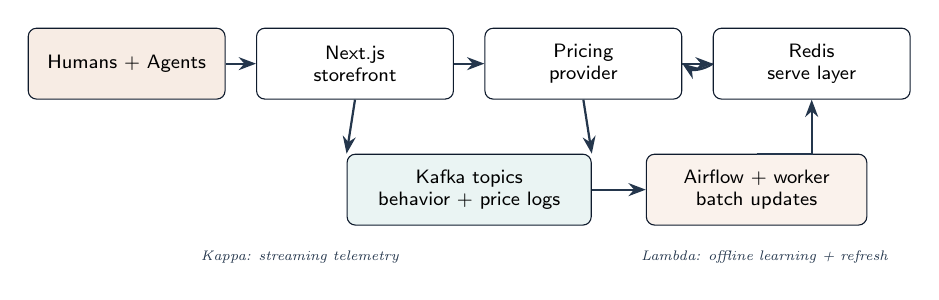
\begin{tikzpicture}[
    font=\scriptsize\sffamily,
    box/.style={draw=PhantomInk,rounded corners=3pt,minimum width=2.5cm,minimum height=0.9cm,align=center},
    arr/.style={-{Stealth[length=2.2mm]},thick,PhantomSlate}
  ]
    \node[box,fill=PhantomCyan!14] (actors) at (0,1.45) {Humans + Agents};
    \node[box,fill=white] (web) at (2.9,1.45) {Next.js\\storefront};
    \node[box,fill=white] (provider) at (5.8,1.45) {Pricing\\provider};
    \node[box,fill=white] (redis) at (8.7,1.45) {Redis\\serve layer};
    \node[box,fill=PhantomIndigo!10,minimum width=3.1cm] (kafka) at (4.35,-0.15) {Kafka topics\\behavior + price logs};
    \node[box,fill=PhantomCyan!10,minimum width=2.8cm] (airflow) at (8.0,-0.15) {Airflow + worker\\batch updates};

    \draw[arr] (actors) -- (web);
    \draw[arr] (web) -- (provider);
    \draw[arr] (provider) -- (redis);
    \draw[arr] (web.south) -- (kafka.north west);
    \draw[arr] (provider.south) -- (kafka.north east);
    \draw[arr] (kafka) -- (airflow);
    \draw[arr] (airflow.north) -| (redis.south);
    \draw[arr] (redis.west) to[bend left=35] (provider.east);

    \node[font=\tiny\itshape,text=PhantomSlate] at (2.2,-1.0) {Kappa: streaming telemetry};
    \node[font=\tiny\itshape,text=PhantomSlate] at (8.1,-1.0) {Lambda: offline learning + refresh};
  \end{tikzpicture}

  \vspace{0.35em}
  \begin{itemize}[<+->]
    \item Every quote has a matching behavioral context in the log stream.
    \item The same architecture supports reproducible stress tests before any live deployment.
  \end{itemize}
  \stagebar{2}
\end{frame}

\begin{frame}{Dataset card: compact, labeled, and experiment-ready}
  \begin{columns}[T,onlytextwidth]
    \column{0.60\textwidth}
    \centering
    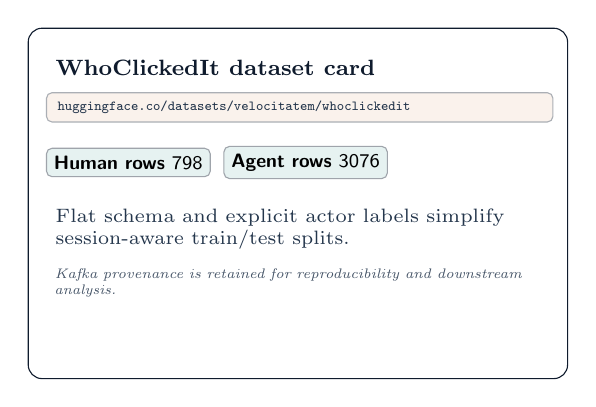
\begin{tikzpicture}[
      font=\scriptsize\sffamily,
      chip/.style={draw=PhantomInk!40,rounded corners=2pt,inner sep=2.7pt},
      body/.style={anchor=west,text width=6.0cm,align=left,font=\scriptsize}
    ]
      \node[draw=PhantomInk,rounded corners=5pt,fill=white,minimum width=6.85cm,minimum height=4.45cm] at (0,0) {};
      \node[anchor=west,font=\footnotesize\bfseries,text=PhantomInk] at (-3.2,1.72) {WhoClickedIt dataset card};
      \node[anchor=west,draw=PhantomInk!35,rounded corners=2pt,fill=PhantomCyan!10,inner xsep=4pt,inner ysep=3pt,text width=6.15cm,align=left,font=\tiny\ttfamily,text=PhantomSlate] at (-3.2,1.22)
        {huggingface.co/datasets/velocitatem/whoclickedit};

      \node[anchor=west,chip,fill=PhantomIndigo!12] (humanrows) at (-3.2,0.52) {\textbf{Human rows} 798};
      \node[anchor=west,chip,fill=PhantomIndigo!12] at ([xshift=0.16cm]humanrows.east) {\textbf{Agent rows} 3076};

      \node[body,text=PhantomSlate] at (-3.2,-0.33)
        {Flat schema and explicit actor labels simplify session-aware train/test splits.};
      \node[body,font=\tiny\itshape,text=PhantomSlate!85] at (-3.2,-1.01)
        {Kafka provenance is retained for reproducibility and downstream analysis.};
    \end{tikzpicture}

    \column{0.38\textwidth}
    \centering
    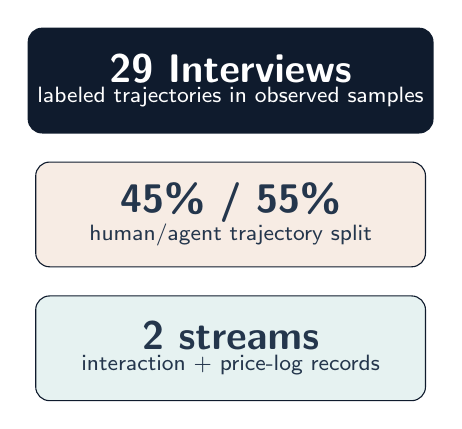
\begin{tikzpicture}[font=\scriptsize\sffamily,
      stat/.style={draw=PhantomInk,rounded corners=5pt,minimum width=4.95cm,minimum height=1.33cm,align=center}]
      \node<1->[stat,fill=PhantomInk,text=white] at (0,1.95)
        {\Large\bfseries 29 Interviews\\[-0.1em]\footnotesize labeled trajectories in observed samples};
      \node<2->[stat,fill=PhantomCyan!14,text=PhantomSlate] at (0,0.25)
        {\Large\bfseries 45\% / 55\%\\[-0.1em]\footnotesize human/agent trajectory split};
      \node<3->[stat,fill=PhantomIndigo!12,text=PhantomSlate] at (0,-1.45)
        {\Large\bfseries 2 streams\\[-0.1em]\footnotesize interaction + price-log records};
    \end{tikzpicture}
  \end{columns}

  \stagebar{2}
\end{frame}

\begin{frame}{Experimental design controls goals, not instructions}
  \begin{columns}[T,onlytextwidth]
    \column{0.58\textwidth}
    \centering
    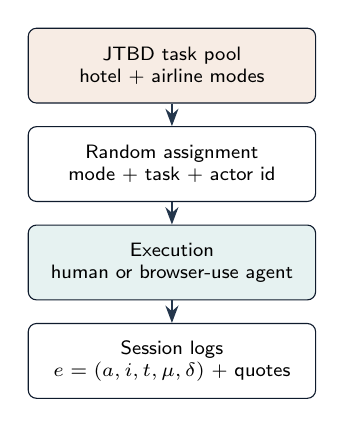
\begin{tikzpicture}[
      font=\scriptsize\sffamily,
      box/.style={draw=PhantomInk,rounded corners=3pt,minimum width=3.65cm,minimum height=0.95cm,align=center},
      arr/.style={-{Stealth[length=2.2mm]},thick,PhantomSlate}
    ]
      \node[box,fill=PhantomCyan!14] (tasks) at (0,1.8) {JTBD task pool\\hotel + airline modes};
      \node[box,fill=white] (assign) at (0,0.55) {Random assignment\\mode + task + actor id};
      \node[box,fill=PhantomIndigo!12] (run) at (0,-0.7) {Execution\\human or browser-use agent};
      \node[box,fill=white] (logs) at (0,-1.95) {Session logs\\$e=(a,i,t,\mu,\delta)$ + quotes};
      \draw[arr] (tasks) -- (assign);
      \draw[arr] (assign) -- (run);
      \draw[arr] (run) -- (logs);
    \end{tikzpicture}

    \column{0.40\textwidth}
    \begin{itemize}[<+->]\setlength{\itemsep}{0.55em}
      \item Agents run with \textbf{browser-use} and a model-swappable LLM router (default \texttt{gpt-5-mini}).
      \item Tasks are defined by outcomes, not scripted clicks, to preserve behavioral variety.
      \item Current release is stronger on hotel flows than airline flows.
    \end{itemize}
  \end{columns}
  \stagebar{2}
\end{frame}

\section{Distinguishability Construction}

\begin{frame}{Stage 2: A behavior kernel is a compact signature of navigation dynamics}
  \begin{columns}[T,onlytextwidth]
    \column{0.48\textwidth}
    \begin{block}{Definition}
      \[
        \hat P(s'\mid s)=\frac{N(s,s')}{\sum_k N(s,k)}
      \]
    \end{block}
    \begin{itemize}[<+->]
      \item Build one kernel per session, then prototypes for human and agent cohorts.
      \item Compare each incoming session to both prototypes with KL divergence.
    \end{itemize}

    \column{0.50\textwidth}
    \centering
    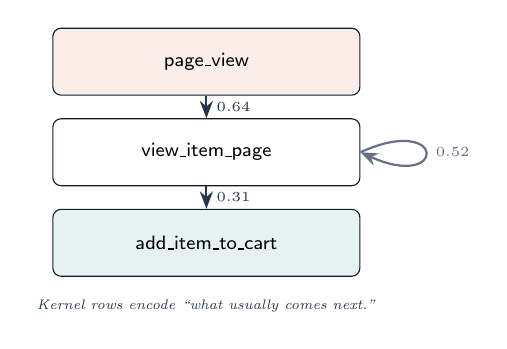
\begin{tikzpicture}[font=\scriptsize\sffamily]
      \node[draw=PhantomInk,rounded corners=3pt,fill=PhantomCyan!12,minimum width=3.9cm,minimum height=0.85cm] (a) at (0,1.4) {page\_view};
      \node[draw=PhantomInk,rounded corners=3pt,fill=white,minimum width=3.9cm,minimum height=0.85cm] (b) at (0,0.25) {view\_item\_page};
      \node[draw=PhantomInk,rounded corners=3pt,fill=PhantomIndigo!12,minimum width=3.9cm,minimum height=0.85cm] (c) at (0,-0.9) {add\_item\_to\_cart};
      \draw[-{Stealth[length=2.2mm]},thick,PhantomSlate] (a) -- node[right,font=\tiny]{0.64} (b);
      \draw[-{Stealth[length=2.2mm]},thick,PhantomSlate] (b) -- node[right,font=\tiny]{0.31} (c);
      \draw[-{Stealth[length=2.2mm]},thick,PhantomSlate!70] (b.east) .. controls +(1.1,0.5) and +(1.1,-0.5) .. node[right,font=\tiny]{0.52} (b.east);
      \node[font=\tiny\itshape,text=PhantomSlate] at (0,-1.7) {Kernel rows encode ``what usually comes next.''};
    \end{tikzpicture}
  \end{columns}
  \stagebar{3}
\end{frame}

\begin{frame}{Human and agent kernels are separable in the controlled cohort}
  \begin{columns}[T,onlytextwidth]
    \column{0.48\textwidth}
    \centering
    \textbf{Human transition structure}\par\vspace{0.2em}
    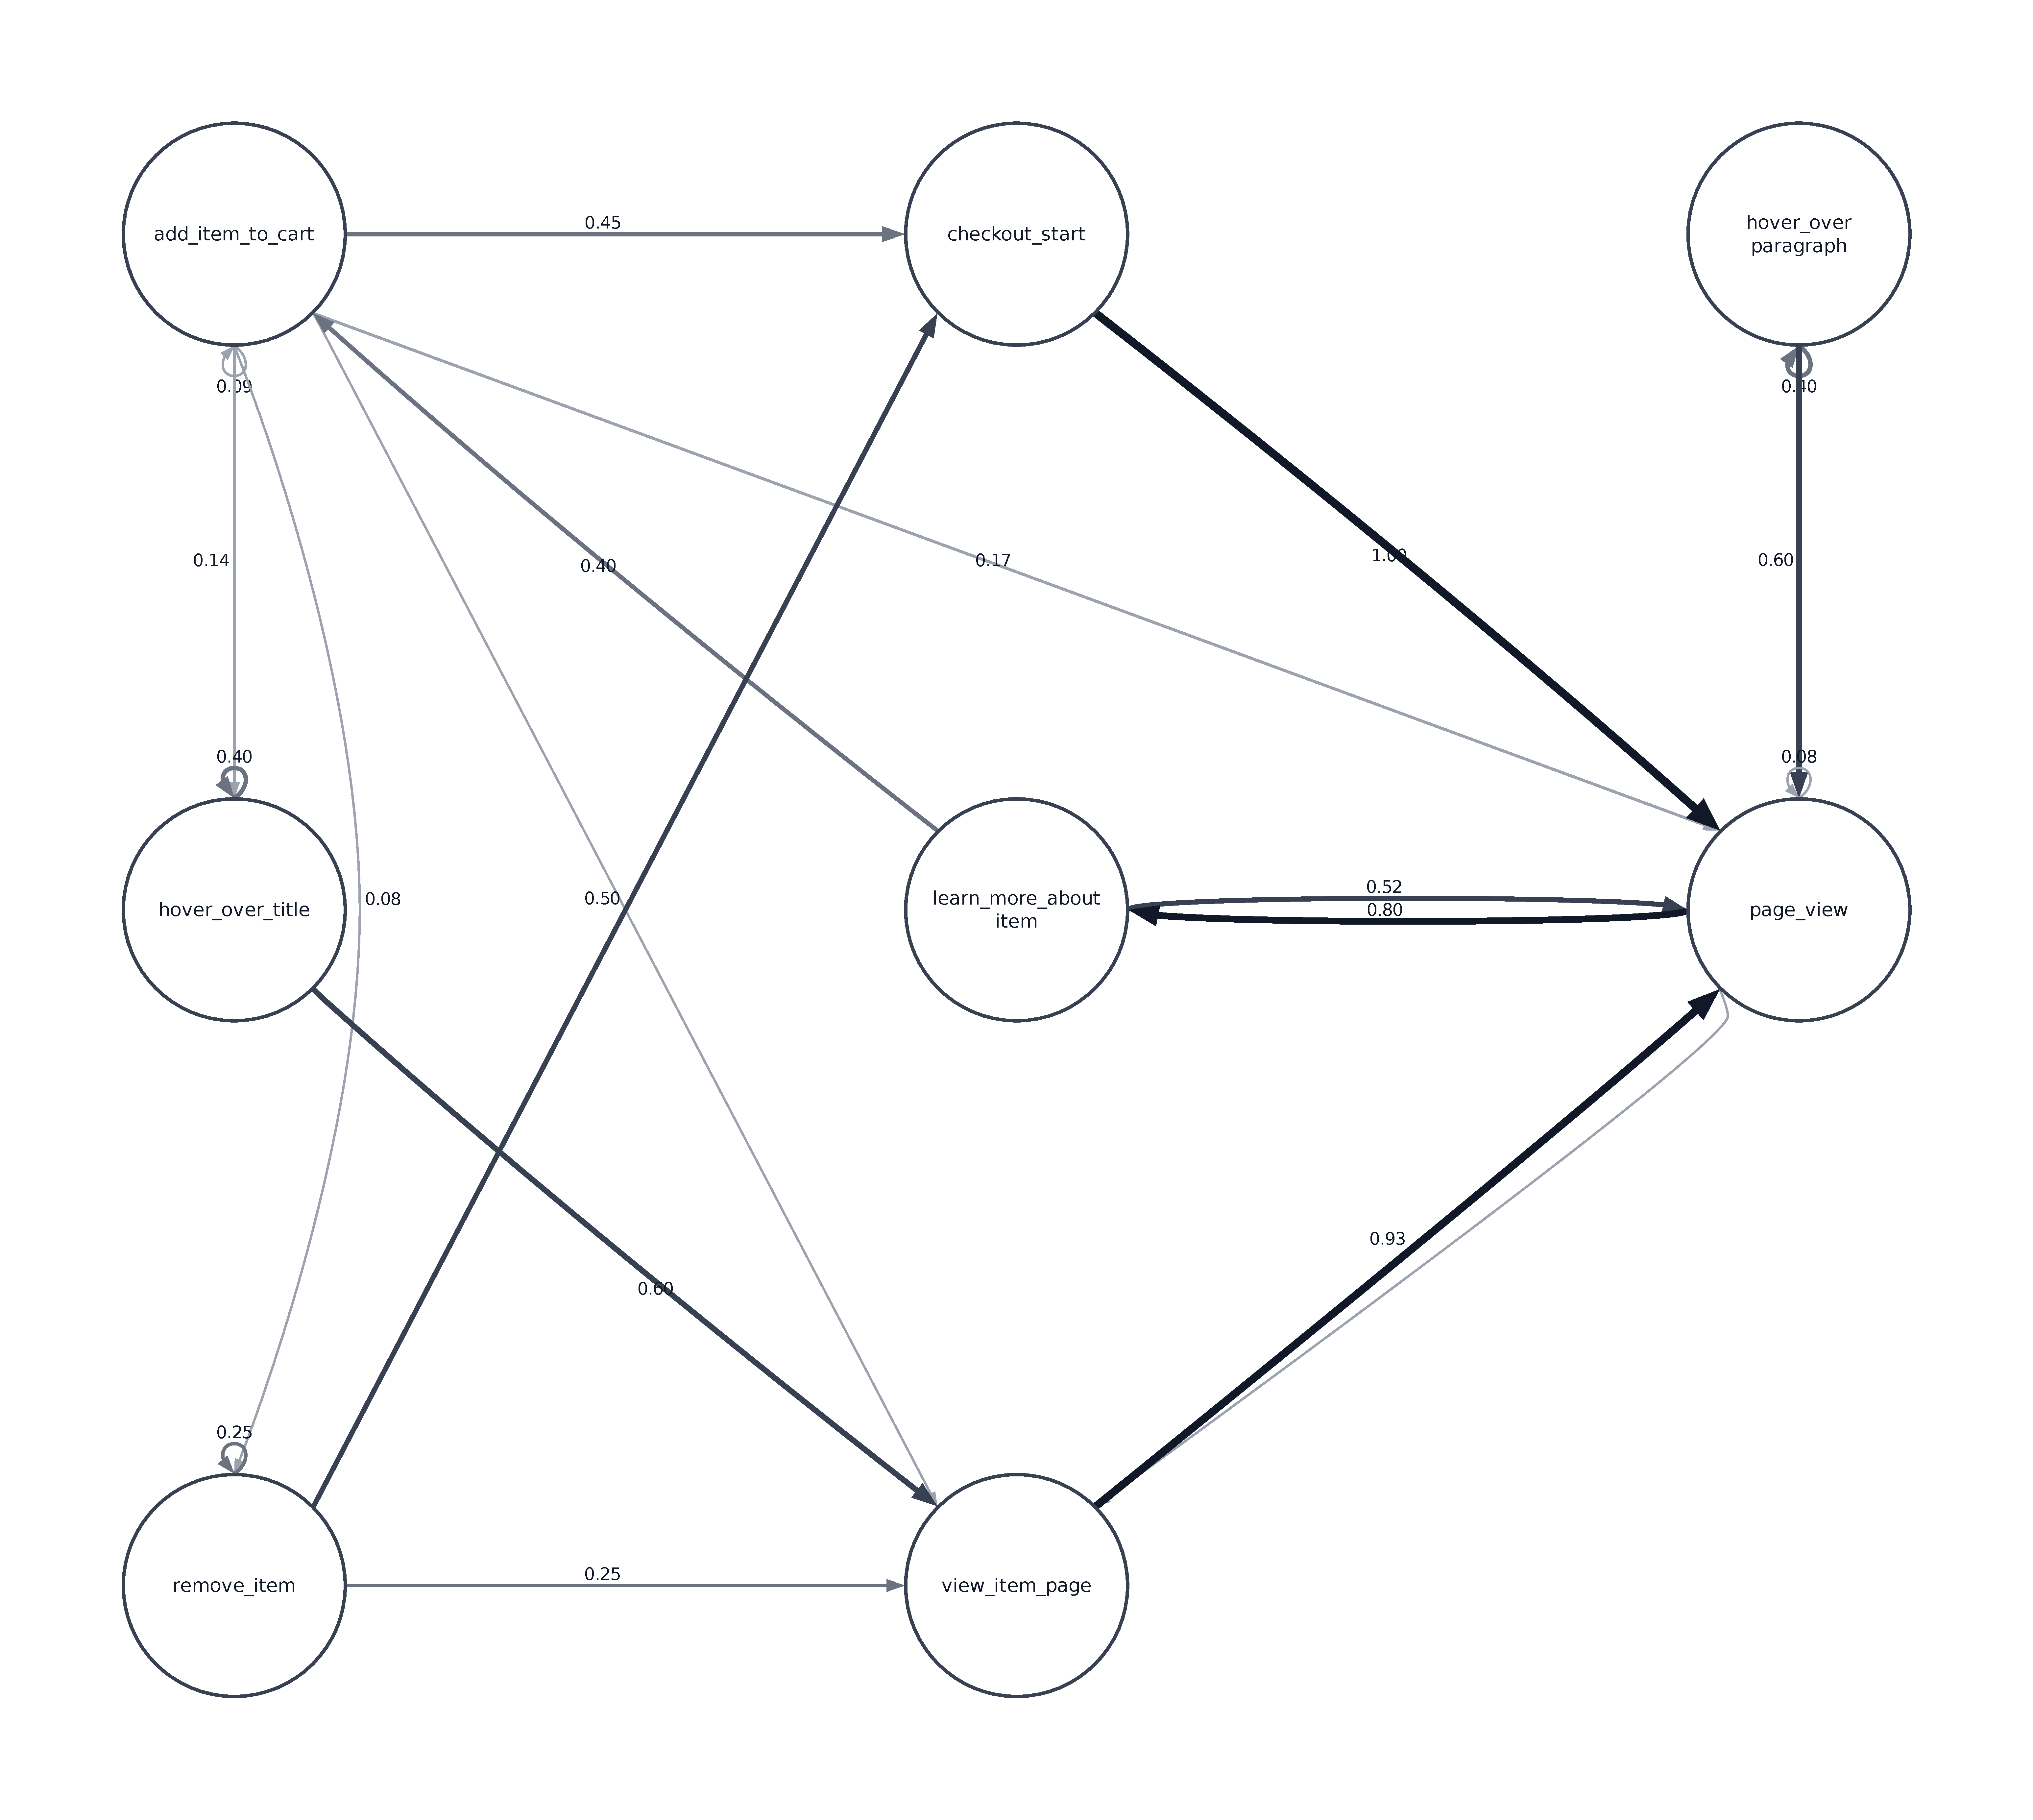
\includegraphics[width=\linewidth,height=0.46\textheight,keepaspectratio]{mdp_human.pdf}
    \column{0.48\textwidth}
    \centering
    \textbf{Agent transition structure}\par\vspace{0.2em}
    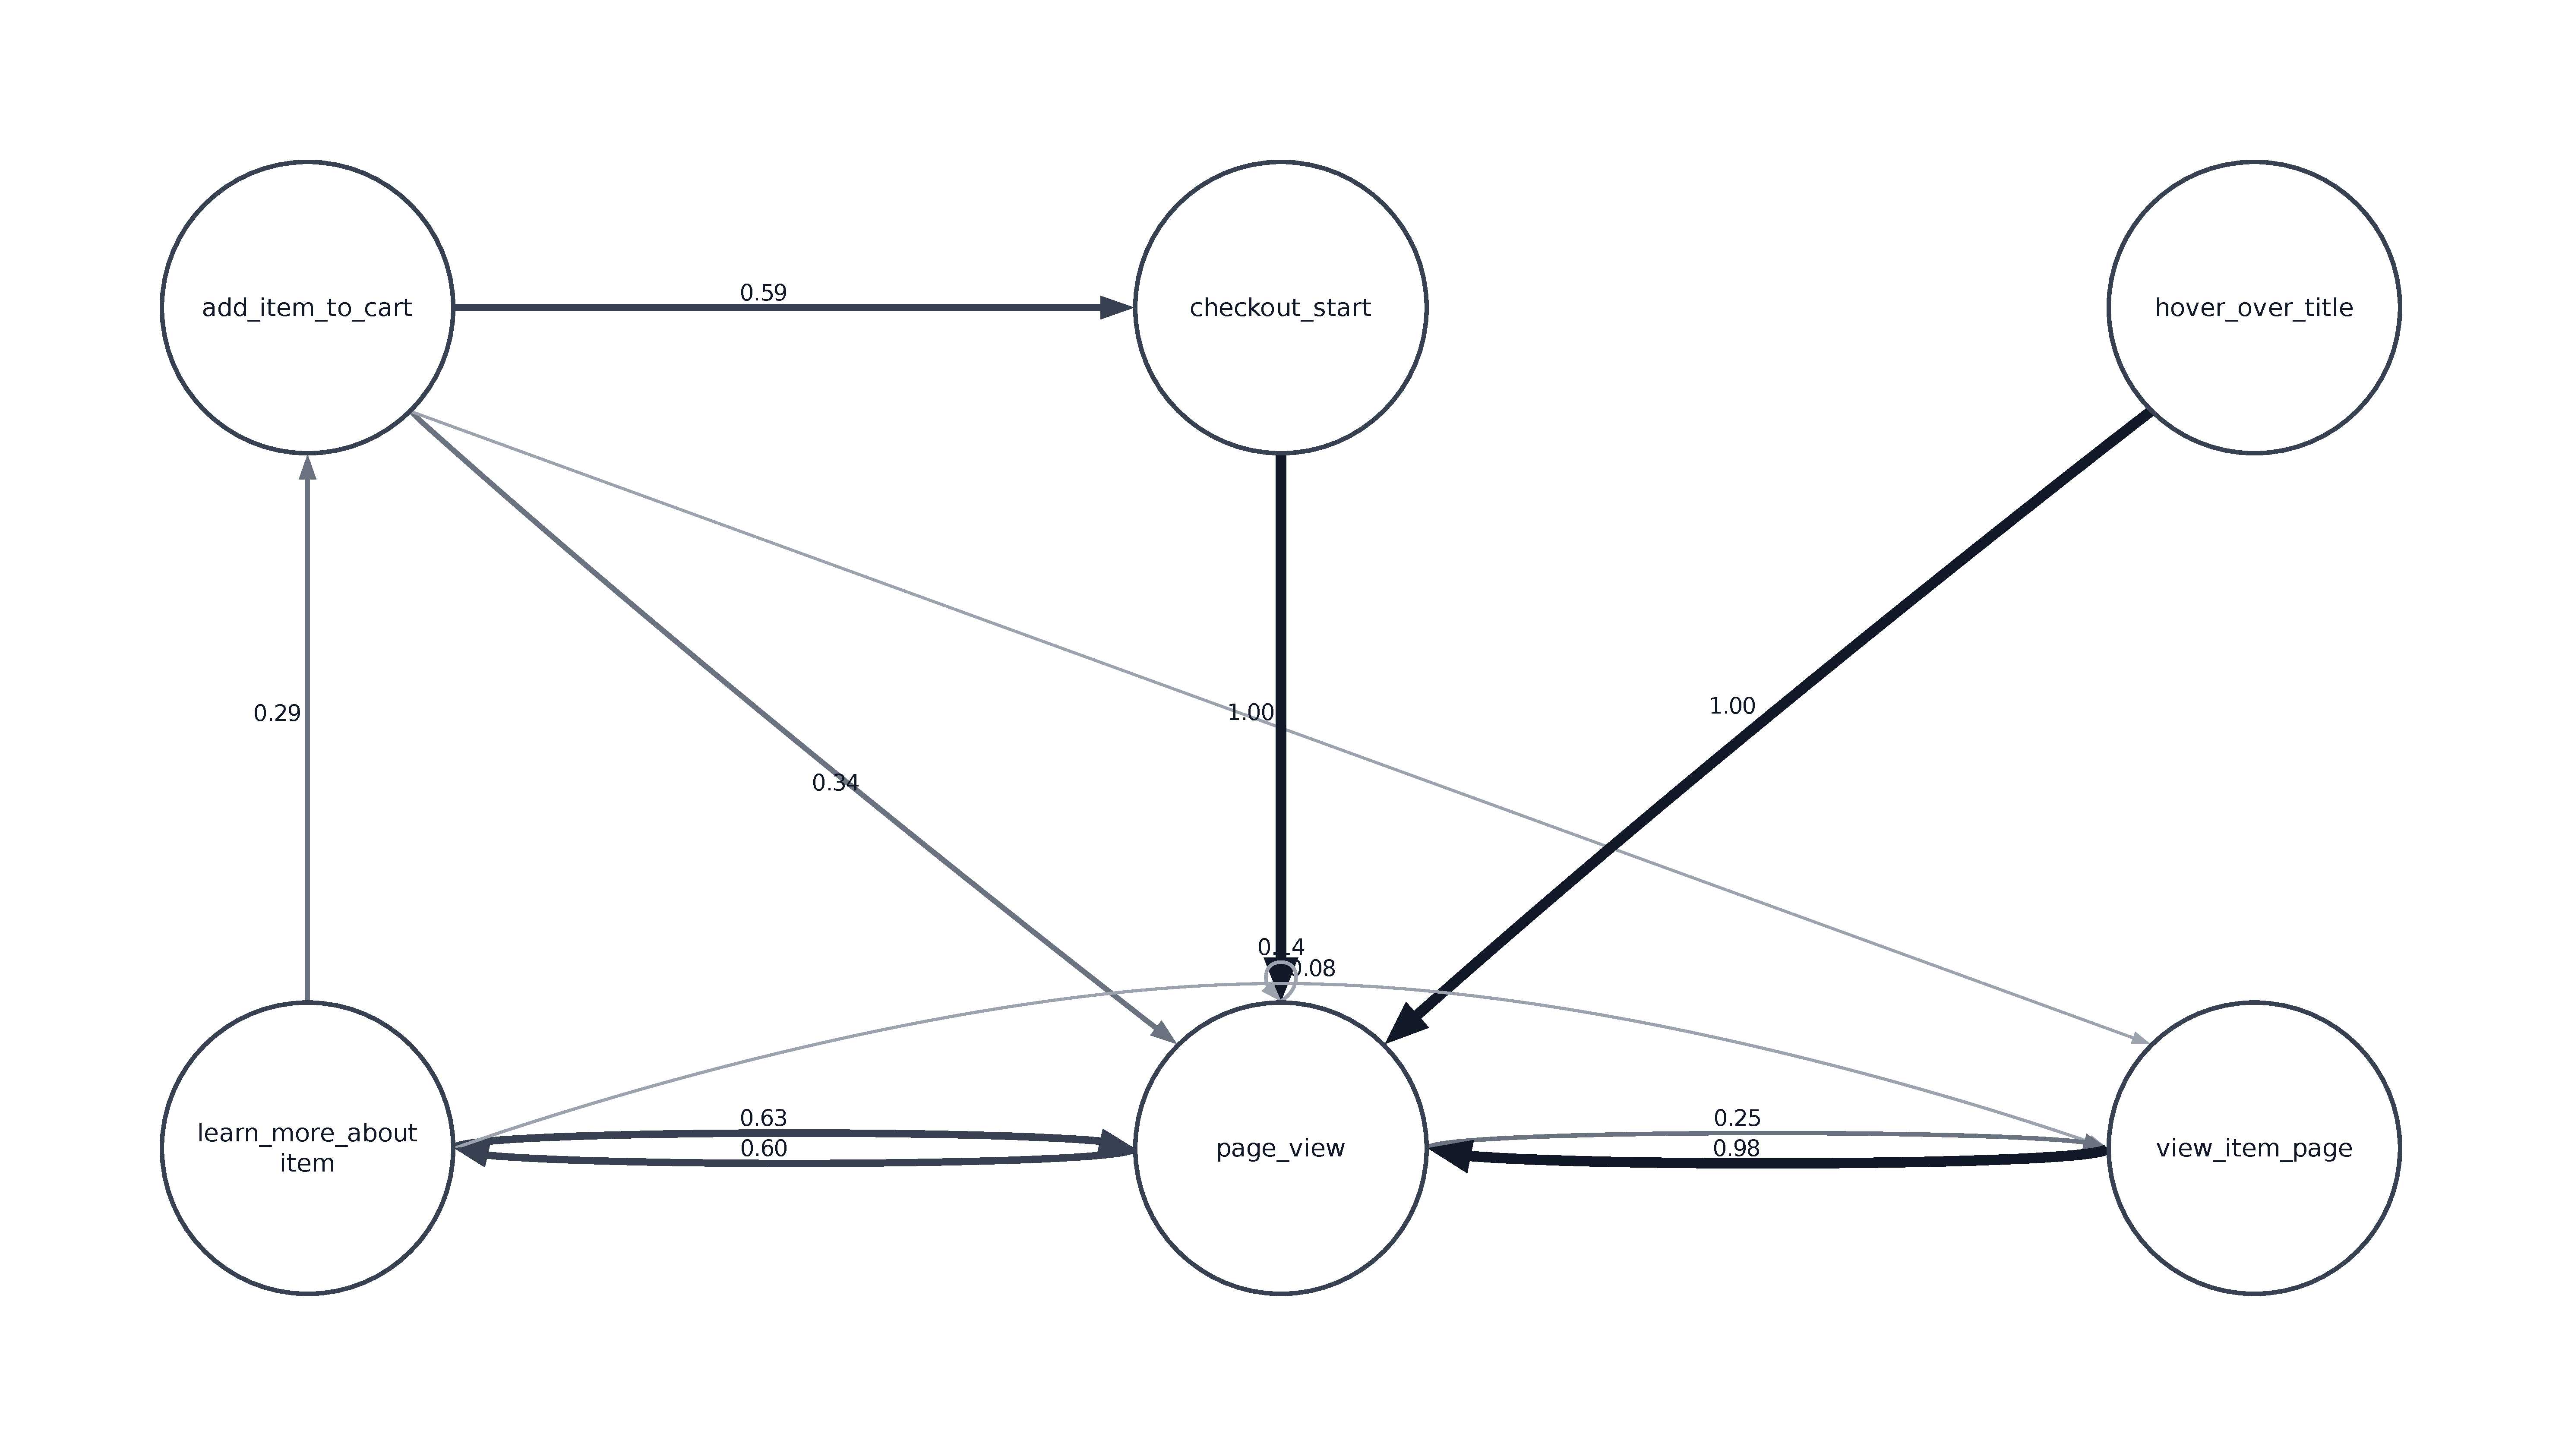
\includegraphics[width=\linewidth,height=0.46\textheight,keepaspectratio]{mdp_agent.pdf}
  \end{columns}

  \vspace{0.15em}
  \begin{columns}[T,onlytextwidth]
    \column{0.32\textwidth}\centering\metriccard{-3.35}{mean gap (human)}
    \column{0.32\textwidth}\centering\metriccard{+1.65}{mean gap (agent)}
    \column{0.32\textwidth}\centering\metriccard{$p<0.001$}{Mann-Whitney rank test}
  \end{columns}
  \stagebar{3}
\end{frame}

\begin{frame}{Two divergence scores become one continuous control signal}
  \centering
  \[
    \only<1>{\Delta_H = D_{KL}(\hat T'\mid\mid\bar T_H),\quad \Delta_A = D_{KL}(\hat T'\mid\mid\bar T_A)}%
    \only<2>{g(\tau') = \Delta_H-\Delta_A}%
    \only<3->{f(\tau') = P(A\mid\tau') = \sigma\!\left(\frac{g(\tau')}{T}\right)}
  \]

  \vspace{0.4em}
  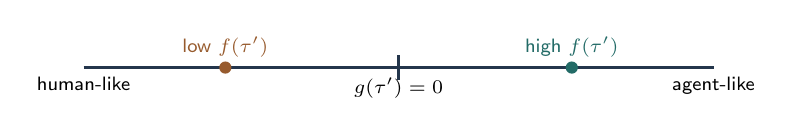
\begin{tikzpicture}[font=\scriptsize\sffamily]
    \draw<2->[very thick,PhantomSlate] (-4,0) -- (4,0);
    \draw<2->[thick,PhantomSlate] (0,-0.16) -- (0,0.16);
    \node<2->[anchor=north] at (-4,0) {human-like};
    \node<2->[anchor=north] at (4,0) {agent-like};
    \node<3->[anchor=north] at (0,0) {$g(\tau')=0$};
    \fill<4->[PhantomCyan!75!black] (-2.2,0) circle (2.2pt);
    \node<4->[anchor=south,text=PhantomCyan!75!black] at (-2.2,0) {low $f(\tau')$};
    \fill<5->[PhantomIndigo!75!black] (2.2,0) circle (2.2pt);
    \node<5->[anchor=south,text=PhantomIndigo!75!black] at (2.2,0) {high $f(\tau')$};
  \end{tikzpicture}

  \vspace{0.25em}
  \begin{itemize}
    \item<3-> The signed gap $g(\tau')$ is positive when a session is closer to agent behavior.
    \item<4-> Temperature $T$ calibrates how sharply the score moves away from uncertainty.
    \item<6-> Continuous scoring is used to steer contamination-aware pricing.
    \item<7-> The design target is guidance, not a hard user-level ban decision.
  \end{itemize}
  \stagebar{3}
\end{frame}

\section{Distributionally Robust RL}

\begin{frame}{Stage 3: DR-RL trains against plausible contamination shifts, not one fixed world}
  \small
  \begin{columns}[T,onlytextwidth]
    \column{0.48\textwidth}
    \begin{block}{Ideal robust object}
      \[
        \mathcal U_\epsilon(\hat P_N)=\{Q: W_p(Q,\hat P_N)\le\epsilon\}
      \]
      \centering
      robust against distribution shift around the empirical demand law
    \end{block}

    \column{0.50\textwidth}
    \begin{block}{Engine approximation used in experiments}
      \[
        \mathcal A_{\epsilon_\alpha}(\alpha_0)=\{\alpha:|\alpha-\alpha_0|\le\epsilon_\alpha\}
      \]
      \centering
      small grid over $\alpha$ \;\textrightarrow\; inner worst-case candidate
    \end{block}
  \end{columns}
  \vspace{0.2em}
  \begin{alertblock}{Practical boundary}
    In code we solve a local robust loop around $\alpha_0$, not the full continuous Wasserstein adversary.
  \end{alertblock}
  \stagebar{4}
\end{frame}

\begin{frame}{Reward composition penalizes leakage while guarding user experience}
  \[
    \only<1>{%
      r_t =
      {\color{PhantomInk}\underline{R(p_t,\hat Q_t)}}%
    }%
    \only<2>{%
      r_t =
      {\color{PhantomInk}\underline{R(p_t,\hat Q_t)}}
      - {\color{PhantomCyan!95!black}\underline{\lambda\,f(\tau'_t)\,c_{\text{info}}}}%
    }%
    \only<3->{%
      r_t =
      {\color{PhantomInk}\underline{R(p_t,\hat Q_t)}}
      - {\color{PhantomCyan!95!black}\underline{\lambda\,f(\tau'_t)\,c_{\text{info}}}}
      - {\color{PhantomIndigo!95!black}\underline{\eta_{\text{ux}}\,UX(\tau'_t,p_t)}}%
    }%
  \]

  \vspace{0.45em}
  \begin{columns}[T,onlytextwidth]
    \column{0.32\textwidth}
    \centering
    
\begin{tikzpicture}[font=\scriptsize\sffamily]
      \node[
        draw=PhantomInk,
        rounded corners=4pt,
        fill=PhantomInk!12,
        minimum width=0.98\linewidth,
        text width=0.88\linewidth,
        minimum height=1.28cm,
        align=center,
        text=PhantomInk
      ] {\textbf{Revenue term}\\[-0.08em]keeps market objective explicit};
    \end{tikzpicture}
    \column{0.32\textwidth}
    \centering
    \uncover<2->{%
      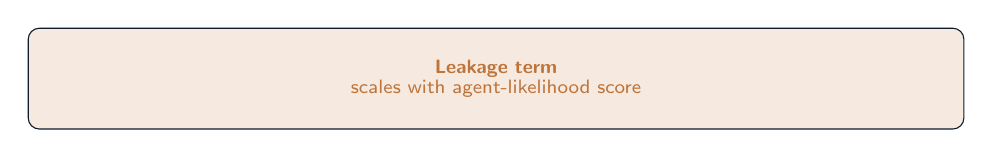
\begin{tikzpicture}[font=\scriptsize\sffamily]
        \node[
          draw=PhantomInk,
          rounded corners=4pt,
          fill=PhantomCyan!16,
          minimum width=0.98\linewidth,
          text width=0.88\linewidth,
          minimum height=1.28cm,
          align=center,
          text=PhantomCyan!95!black
        ] {\textbf{Leakage term}\\[-0.08em]scales with agent-likelihood score};
      \end{tikzpicture}%
    }
    \column{0.32\textwidth}
    \centering
    \uncover<3->{%
      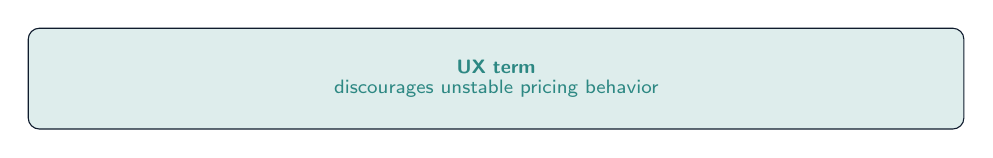
\begin{tikzpicture}[font=\scriptsize\sffamily]
        \node[
          draw=PhantomInk,
          rounded corners=4pt,
          fill=PhantomIndigo!16,
          minimum width=0.98\linewidth,
          text width=0.88\linewidth,
          minimum height=1.28cm,
          align=center,
          text=PhantomIndigo!95!black
        ] {\textbf{UX term}\\[-0.08em]discourages unstable pricing behavior};
      \end{tikzpicture}%
    }
  \end{columns}

  \vspace{0.25em}
  \begin{itemize}
    \item<2-> Baseline experiments use a query-tax leakage surrogate for tractability.
    \item<3-> Supra-competitive anchor penalties are tracked as an additional safety rail.
  \end{itemize}
  \stagebar{4}
\end{frame}

\begin{frame}{Computationally, wide sweeps are feasible only with aggressive optimization}
  \begin{columns}[T,onlytextwidth]
    \column{0.47\textwidth}
    \centering
    {\Large\(4\times4\times3\times2\times2=\mathbf{192}\)}\\[0.25em]
    {\scriptsize algorithms $\times$ contamination $\times$ robustness $\times$ COI penalty $\times$ action grid}

    \vspace{0.5em}
    \metriccard{160 PFLOPS}{peak aggregate TPU budget}\\[0.45em]
    \metriccard{\textasciitilde180 days}{net compute logged in full study}

    \column{0.51\textwidth}
    \begin{block}{Hot-path rewrite impact}
      \centering
      \begin{tabular}{@{}lcc@{}}
        \toprule
        Mode & Before & After \\
        \midrule
        Baseline step/s & 26.0 & 220.0 \\
        Robust step/s & 7.2 & 136.0 \\
        \bottomrule
      \end{tabular}
    \end{block}
    \vspace{0.1em}
    {\footnotesize
    \begin{itemize}[<+->]
      \item pandas lookup bottlenecks replaced with array/JAX-style loops.
      \item Throughput gains (8.5$\times$, 19$\times$) made broad sweeps practical.
    \end{itemize}}
  \end{columns}
  \stagebar{4}
\end{frame}

\section{Results}

\begin{frame}{Results: contamination hurts revenue; defended policies recover COI}
  \begin{columns}[T,onlytextwidth]
    \column{0.62\textwidth}
    \centering
    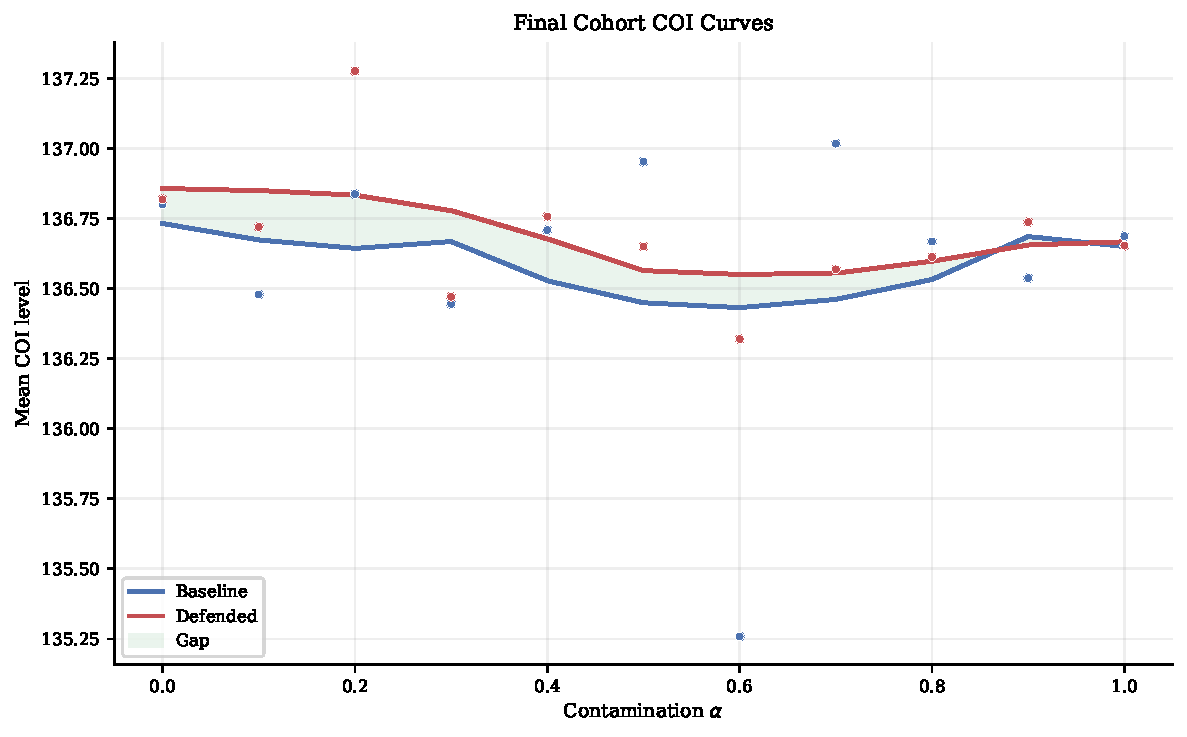
\includegraphics[width=\linewidth,height=0.60\textheight,keepaspectratio]{final_focus_coi_by_alpha.pdf}

    \column{0.30\textwidth}
    \metriccard{-90{,}140}{baseline contamination slope}\\[0.3em]
    \metriccard{\textasciitilde3\%}{short-run revenue cost of defense}\\[0.3em]
    \metriccard{Regime-dependent}{COI gains strongest at harder settings}
  \end{columns}
  \stagebar{5}
\end{frame}

\section{Conclusions}

\begin{frame}{Yes, with boundaries: we can defend margin integrity under agentic orchestration}
  \begin{columns}[T,onlytextwidth]
    \column{0.32\textwidth}
    \begin{block}{SQ1\;Distinguishability}
      \centering
      kernels are separable\\$p<0.001$
    \end{block}
    \column{0.32\textwidth}
    \begin{block}{SQ2\;Theoretical impact}
      \centering
      COI erosion mechanism\\proved in baseline limit
    \end{block}
    \column{0.32\textwidth}
    \begin{block}{SQ3\;Mitigation}
      \centering
      robust control shifts\\COI/revenue/UX trade-off
    \end{block}
  \end{columns}

  \vspace{0.35em}
  \begin{alertblock}{Boundary conditions}
    Evidence is from a controlled platform and a small labeled cohort; this is mechanism validation, not full production external validity.
  \end{alertblock}
  \stagebar{6}
\end{frame}

\begin{frame}{What this implies for real pricing systems}
  \begin{itemize}[<+->]\setlength{\itemsep}{0.7em}
    \item \textbf{Financially:} untreated reconnaissance behaves like an information leak and can compress sustainable margins.
    \item \textbf{Operationally:} behavior-only session scoring can be wired into pricing without relying on device fingerprinting.
    \item \textbf{Market exposure:} channels where dynamic pricing has been a secondary layer (aggregators, comparison funnels, promo traffic) are likely to be disrupted first.
    \item \textbf{Strategically:} robust pricing should be calibrated by regime; there is no single penalty that wins everywhere.
    \item \textbf{Before deployment:} larger human baselines, governance review, and legal safeguards are mandatory.
  \end{itemize}
  \stagebar{6}
\end{frame}

\begin{frame}[plain]
  \centering
  \vfill
  {\LARGE\bfseries Thank you}
  \vspace{0.8em}

  {\large Questions and discussion}

  \vfill
  {\footnotesize\color{PhantomSlate!80}Appendix follows: COI theorem derivation, reward composition, and sample-size notes.}
  \vfill
\end{frame}

\appendix
% Included by defense.tex after the main deck (extensive appendix).

\section{Appendix}

\begin{frame}{Appendix roadmap}
  \footnotesize
  \begin{columns}[T,onlytextwidth]
    \column{0.31\textwidth}
    \begin{block}{A.\ Objects}
      Notation, COI, proxies
    \end{block}
    \column{0.31\textwidth}
    \begin{block}{B.\ Mechanism}
      Order stats, kernels, KL
    \end{block}
    \column{0.31\textwidth}
    \begin{block}{C.\ Control}
      Simulator, robust loop, factorial grid
    \end{block}
  \end{columns}
  \vfill
  \begin{alertblock}{Figures}
    Full charts, MDPs, extra revenue view
  \end{alertblock}
\end{frame}

% ----- A. Notation & definitions -----

\begin{frame}{Appendix: core notation (quick reference, I)}
  \scriptsize
  \begin{align*}
    \tau_s &= (e_{s,1},\ldots,e_{s,L_s}) && \text{session} \\
    \hat{q}_{t,i} &= \sum_{s\in S_t}\sum_k \omega(a_{s,k})\,\mathbf{1}[i_{s,k}=i] && \text{proxy} \\
    Q(p) &= (1-\alpha)\,\mathbb{E}_{\theta\sim D_H}[d(p;\theta)] \\
         &\quad + \alpha\,\mathbb{E}_{\theta\sim D_A}[d(p;\theta)] + \epsilon_t && \text{mixture} \\
    \mathrm{COI}(\pi) &= \mathbb{E}[P]-\underline{p} && \text{COI}
  \end{align*}
\end{frame}

\begin{frame}{Appendix: core notation (quick reference, II)}
  \footnotesize
  \begin{itemize}
    \item \(\underline{p}\): minimum viable price anchor (thesis simplification).
    \item \(\alpha\): contamination with agent traffic in the mixture.
    \item \(\omega(a)\): hand-engineered action weights for the proxy (baseline).
  \end{itemize}
  \begin{alertblock}{Reading guide}
    Objects on the left are \textbf{observable}; \(d(\cdot)\) and many \(\theta\) remain hidden.
  \end{alertblock}
\end{frame}

\begin{frame}{Appendix: COI as a reporting functional}
  \[
    \mathrm{COI}(\pi) = \mathbb{E}_{P\sim F_\pi}[P] - \underline{p}
  \]
  \begin{block}{Interpretation}
    Premium above the floor induced by policy \(\pi\); used as a KPI and as the object Theorem 1 attacks under query saturation.
  \end{block}
\end{frame}

\begin{frame}{Appendix: demand proxy vs.\ latent demand}
  \[
    \hat{q}_{t,i}=\sum_{s\in S_t}\sum_{k=1}^{L_s} \omega(a_{s,k})\,\mathbf{1}[i_{s,k}=i]
  \]
  \begin{alertblock}{Key distinction}
    \(\hat{q}\) is an operational sensor from logs; true demand \(d(p;\theta)\) stays latent. Pricing reacts to \(\hat{q}\), so agent-shaped behavior poisons the signal.
  \end{alertblock}
\end{frame}

% ----- B. Mechanism -----

\begin{frame}{Appendix: independent draws and order statistics (intuition)}
  \begin{columns}[T]
    \column{0.55\textwidth}
    \begin{itemize}
      \item Independent price draws \(\{P_i\}_{i=1}^N\) from fixed offer law.
      \item Purchase-side minimum behaves like \(P_{(1)}\): mass shifts left as \(N\) grows.
      \item Expected premium vs.\ \(\underline{p}\) compresses: COI pressure.
    \end{itemize}
    \column{0.42\textwidth}
    \centering
    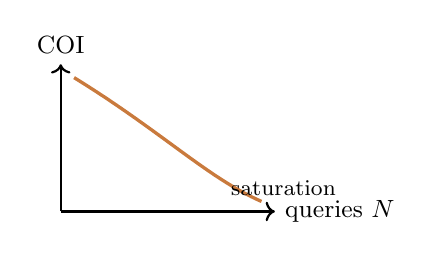
\begin{tikzpicture}[scale=0.85]
      \draw[->,thick] (0,0)--(3.2,0) node[right] {\small queries \(N\)};
      \draw[->,thick] (0,0)--(0,2.2) node[above] {\small COI};
      \draw[PhantomCyan,very thick] (0.2,2) .. controls (1.5,1.2) and (2.2,0.5) .. (3,0.15);
      \node[below right] at (2.4,0.6) {\footnotesize saturation};
    \end{tikzpicture}
  \end{columns}
\end{frame}

\begin{frame}{Appendix: Theorem 1 scope (what is and is not claimed)}
  \small
  \begin{block}{Inside the baseline proof}
    Non-collusive sessions, independent draws, fixed offer distribution across queries.
  \end{block}
  \begin{alertblock}{Outside (handled elsewhere)}
    Collusion, pooled recon, sequential repricing that breaks iid structure: evidence moves to the simulator.
  \end{alertblock}
\end{frame}

\begin{frame}{Appendix: empirical transition kernel (MLE)}
  \[
    \hat{P}(s'\mid s)=\frac{N(s,s')}{\sum_k N(s,k)}
  \]
  \begin{block}{Use}
    Human and agent centroids \(\bar{T}_H,\bar{T}_A\) for divergence-to-prototype scores.
  \end{block}
\end{frame}

\begin{frame}{Appendix: KL to prototypes (shared support)}
  \[
    \Delta_H = D_{\mathrm{KL}}(\hat{T}'\,\|\,\bar{T}_H),\qquad
    \Delta_A = D_{\mathrm{KL}}(\hat{T}'\,\|\,\bar{T}_A)
  \]
  \begin{exampleblock}{Asymmetric choice}
    KL measures deviation from the \textbf{human} reference; symmetric JS/Wasserstein on behavior was not the design target.
  \end{exampleblock}
\end{frame}

\begin{frame}{Appendix: softmax to sigmoid (algebra)}
  \small
  Let \(z_A=-\Delta_A/T\), \(z_H=-\Delta_H/T\). Then
  \begin{align*}
    P(A\mid\tau) &= \frac{e^{z_A}}{e^{z_A}+e^{z_H}}
    = \frac{1}{1+e^{z_H-z_A}}
    = \sigma\bigl(z_A-z_H\bigr) \\
    &= \sigma\!\left(\frac{\Delta_H-\Delta_A}{T}\right).
  \end{align*}
  \begin{block}{Takeaway}
    Two-class softmax over \((z_A,z_H)\) is exactly one sigmoid on the gap \((\Delta_H-\Delta_A)\).
  \end{block}
\end{frame}

\begin{frame}{Appendix: contamination generator \(\mathcal{G}(\alpha)\)}
  \[
    \mathcal{G}(\alpha):\ \text{inject synthetic agent trajectories until mixture reaches target }\alpha
  \]
  \begin{alertblock}{Role in the lab}
    Supplies controlled stress tests for the pricing learner; not a claim of production-faithful agents.
  \end{alertblock}
\end{frame}

% ----- C. Robust control -----

\begin{frame}{Appendix: Wasserstein ambiguity (ideal object)}
  \[
    \mathcal{U}_\epsilon(\hat{P}_N)=\left\{ Q:\ W_p(Q,\hat{P}_N)\le \epsilon \right\}
  \]
  \begin{block}{What the code implements instead}
    A \textbf{local} grid over \(\alpha\) near \(\alpha_0\) with radius \(\epsilon_\alpha\): tractable inner worst case, not a full ball solver.
  \end{block}
\end{frame}

\begin{frame}{Appendix: per-step reward sketch}
  \small
  \[
    r = R(p,d) - \lambda\,\mathrm{COI}_{\mathrm{leak}}(p,\tau') - \eta\,\mathrm{UX}(\tau',p) - \text{(supra-competitive excess)}
  \]
  \begin{itemize}
    \item Query-tax style \(\mathrm{COI}_{\mathrm{leak}}\): minimal nonzero surrogate to expose the control channel.
    \item UX and anchor penalties prevent trivial solutions (flat but exploitative prices).
  \end{itemize}
\end{frame}

\begin{frame}{Appendix: factorial design (192 cells)}
  \footnotesize
  \centering
  \begin{tabular}{@{}llr@{}}
    \toprule
    Axis & Levels & Count \\
    \midrule
    RL algorithm & PPO, A2C, DQN, Q-table & 4 \\
    Contamination \(\alpha\) & 4 representative values in \([0.1,0.6]\) & 4 \\
    Robustness radius \(\epsilon_\alpha\) & 3 & 3 \\
    COI penalty \(\lambda_{\mathrm{coi}}\) & 2 & 2 \\
    Action granularity & 2 & 2 \\
    \midrule
    \textbf{Total} & & \(4\times4\times3\times2\times2=\mathbf{192}\) \\
    \bottomrule
  \end{tabular}
\end{frame}

\begin{frame}{Appendix: engineering note (pandas \(\to\) JAX)}
  \begin{itemize}
    \item Hot path was label-indexed transition lookups; profiling showed pandas overhead dominated.
    \item Integer-indexed arrays + JAX inner loop: large step/s throughput (thesis numbers; environment dependent).
    \item Kronecker expansion of product-conditioned kernels: research simulator cost, scales with catalog.
  \end{itemize}
\end{frame}

% ----- Extended figures (all PDFs in repo) -----

\begin{frame}{Appendix figure: COI by \(\alpha\) (full)}
  \centering
  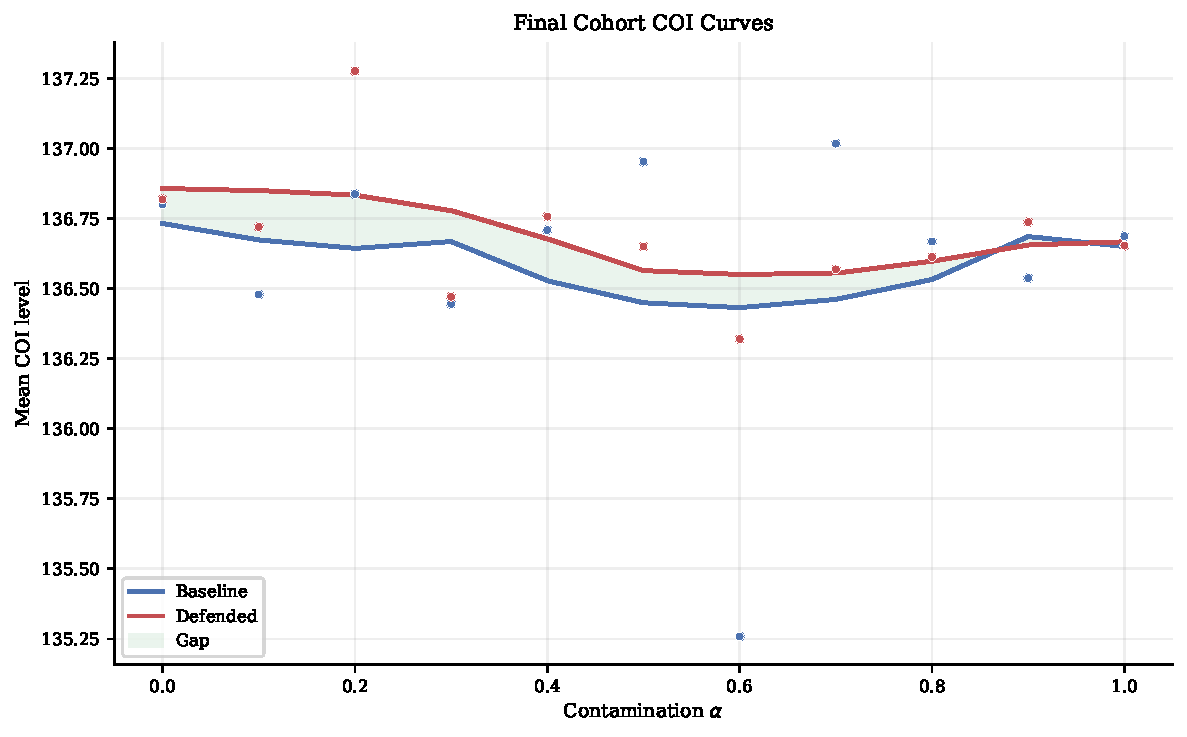
\includegraphics[width=0.92\linewidth,height=0.78\textheight,keepaspectratio]{final_focus_coi_by_alpha.pdf}
\end{frame}

\begin{frame}{Appendix figure: revenue deltas (full)}
  \centering
  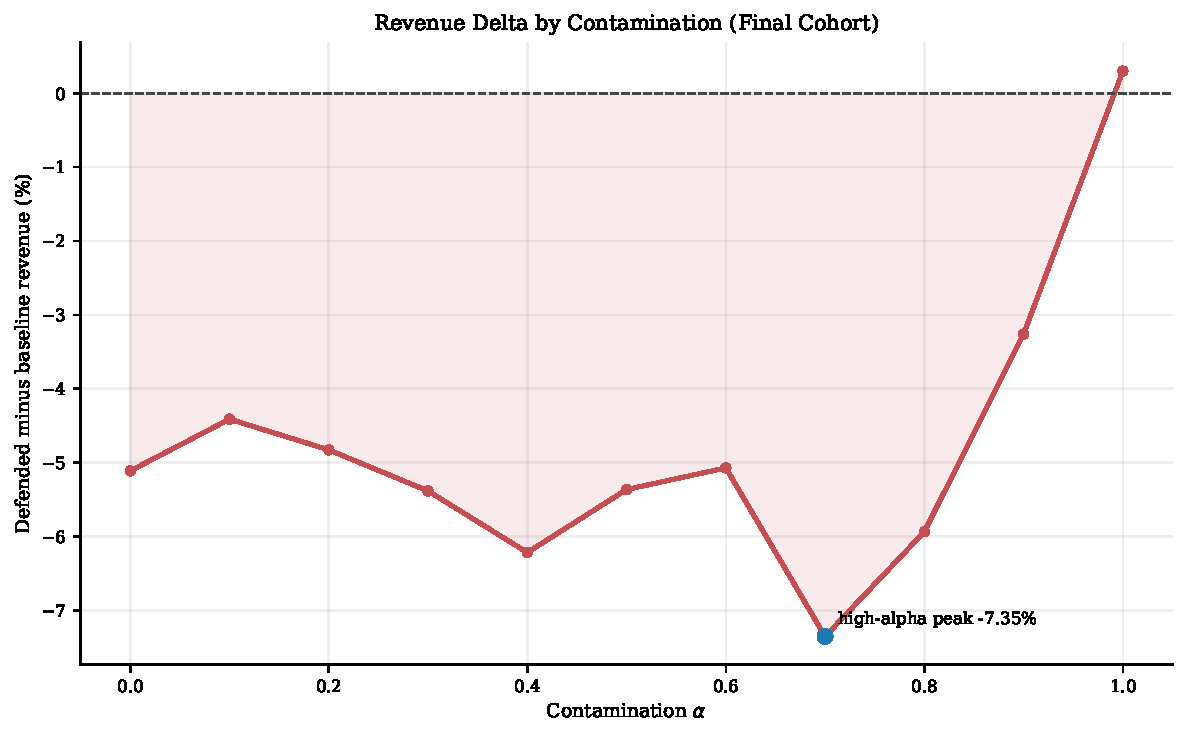
\includegraphics[width=0.92\linewidth,height=0.78\textheight,keepaspectratio]{final_focus_revenue_delta.pdf}
\end{frame}

\begin{frame}{Appendix figure: revenue by \(\alpha\) (full)}
  \centering
  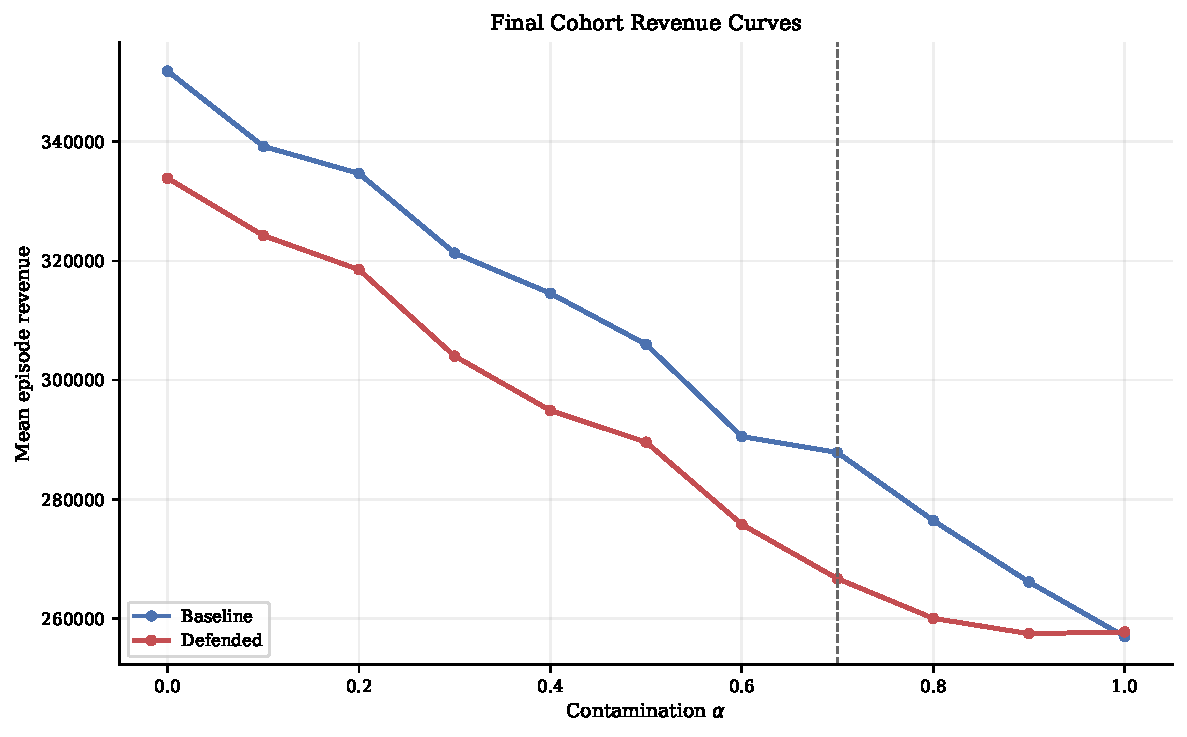
\includegraphics[width=0.92\linewidth,height=0.78\textheight,keepaspectratio]{final_focus_revenue_by_alpha.pdf}
\end{frame}

\begin{frame}{Appendix figure: risk / stability deltas (full)}
  \centering
  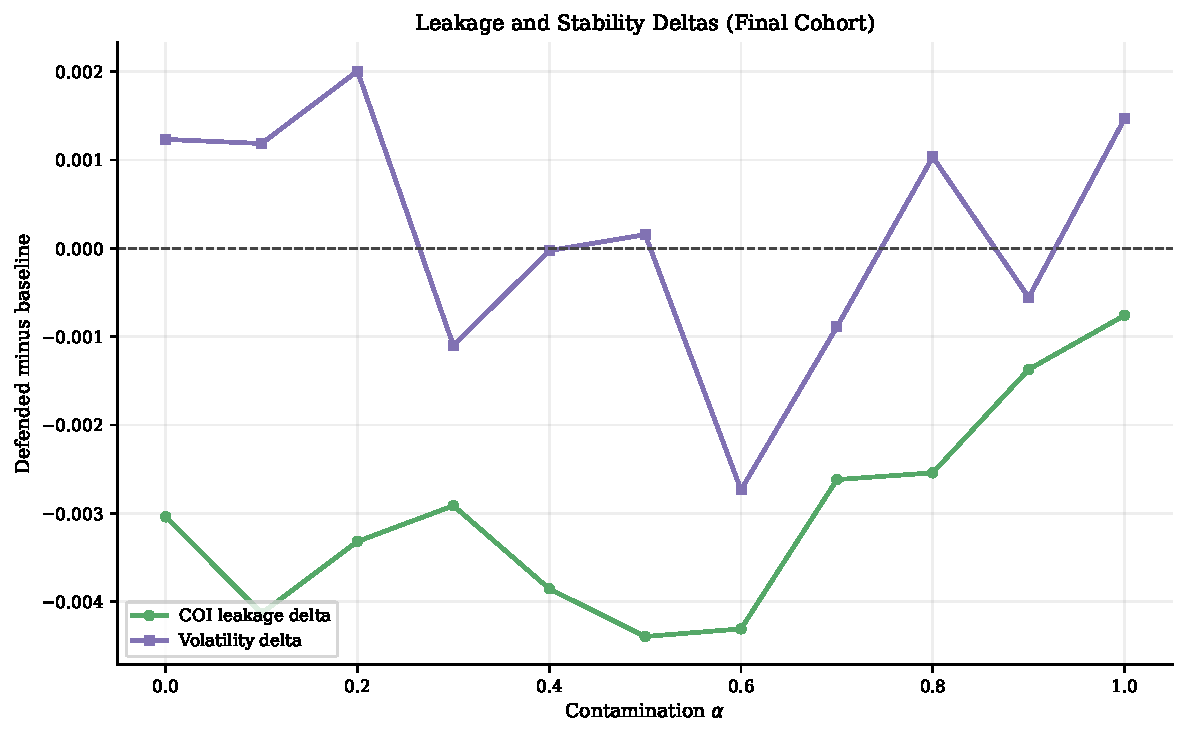
\includegraphics[width=0.92\linewidth,height=0.78\textheight,keepaspectratio]{final_focus_risk_deltas.pdf}
\end{frame}

\begin{frame}{Appendix figure: COI preservation grid (full)}
  \centering
  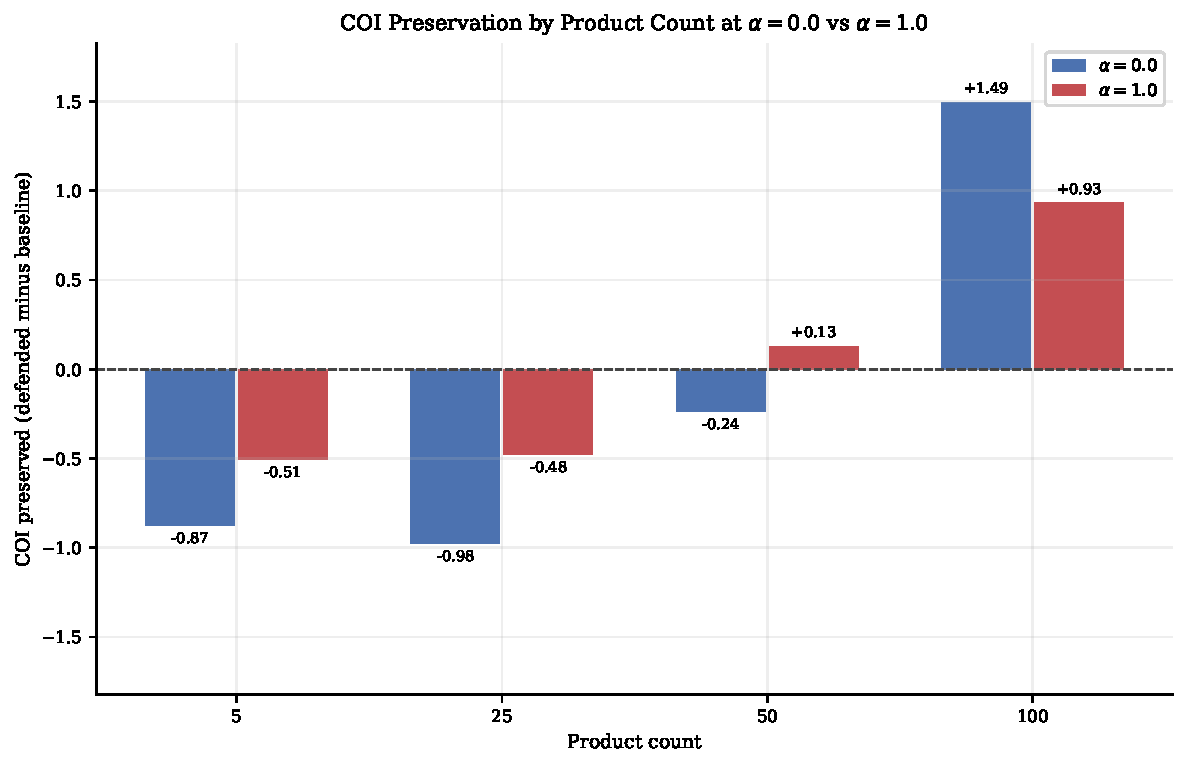
\includegraphics[width=0.92\linewidth,height=0.78\textheight,keepaspectratio]{final_focus_coi_preservation_grid.pdf}
\end{frame}

\begin{frame}{Appendix figure: human MDP (full)}
  \centering
  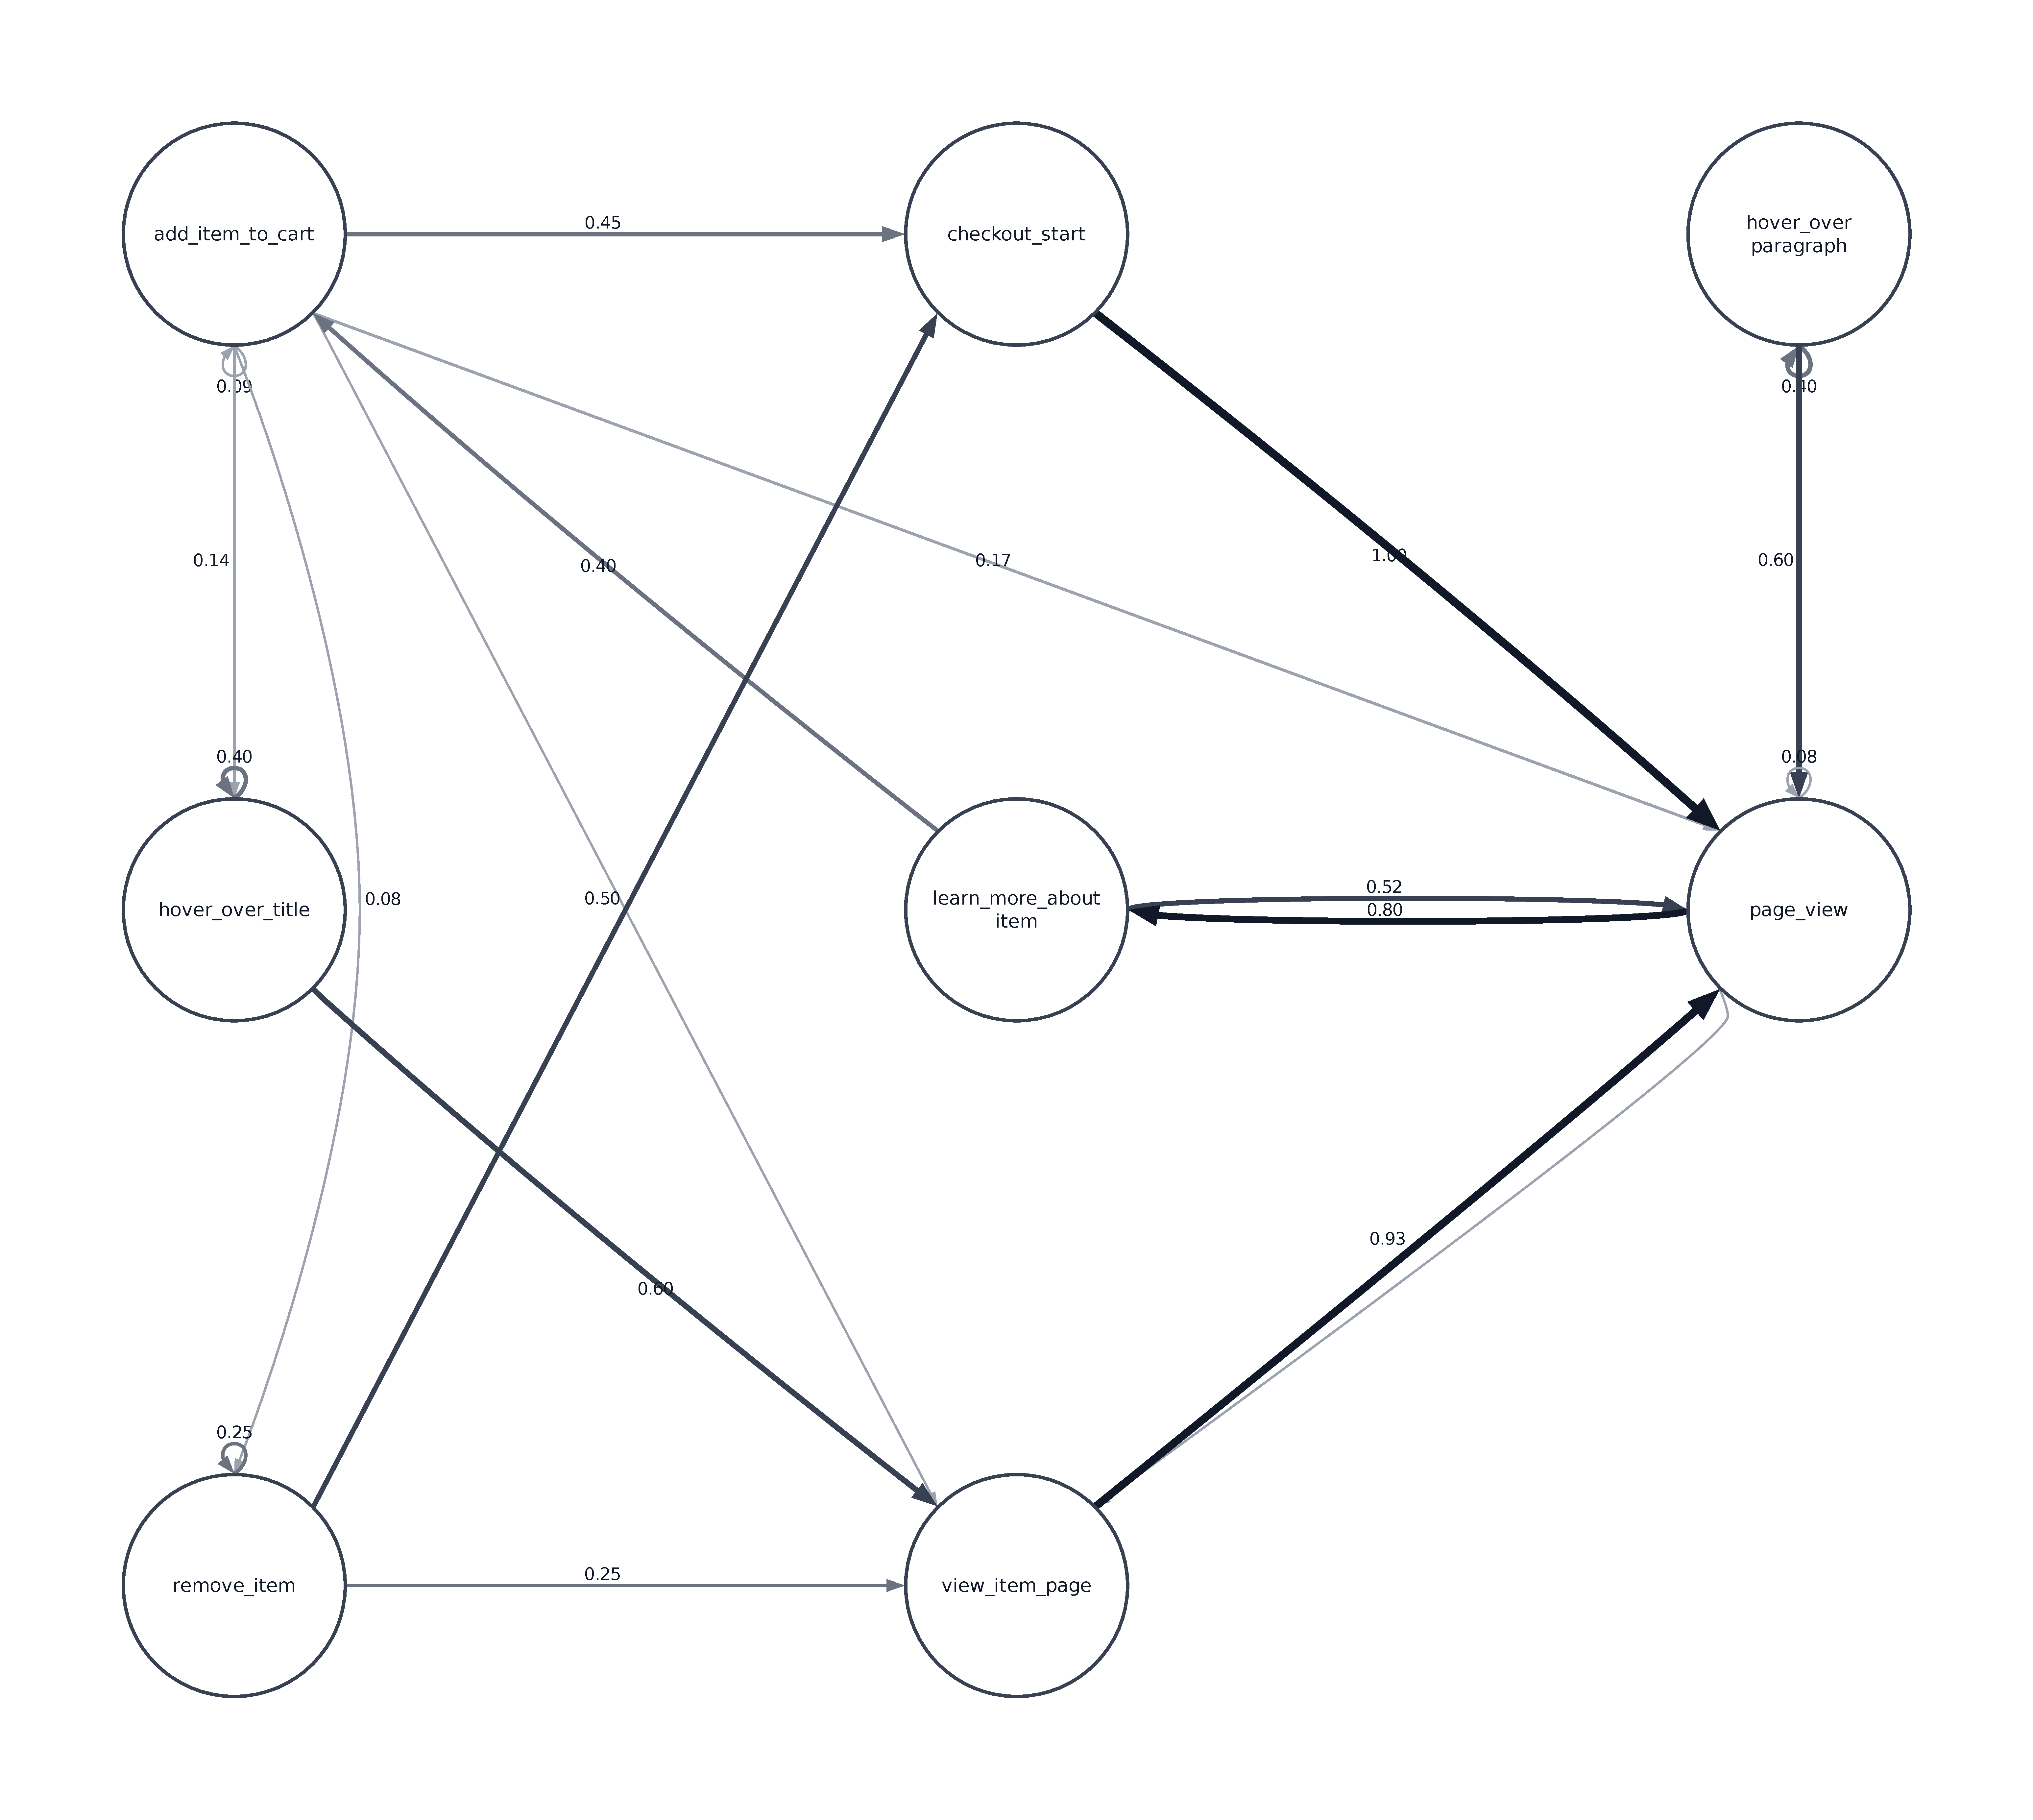
\includegraphics[width=0.75\linewidth,height=0.82\textheight,keepaspectratio]{mdp_human.pdf}
\end{frame}

\begin{frame}{Appendix figure: agent MDP (full)}
  \centering
  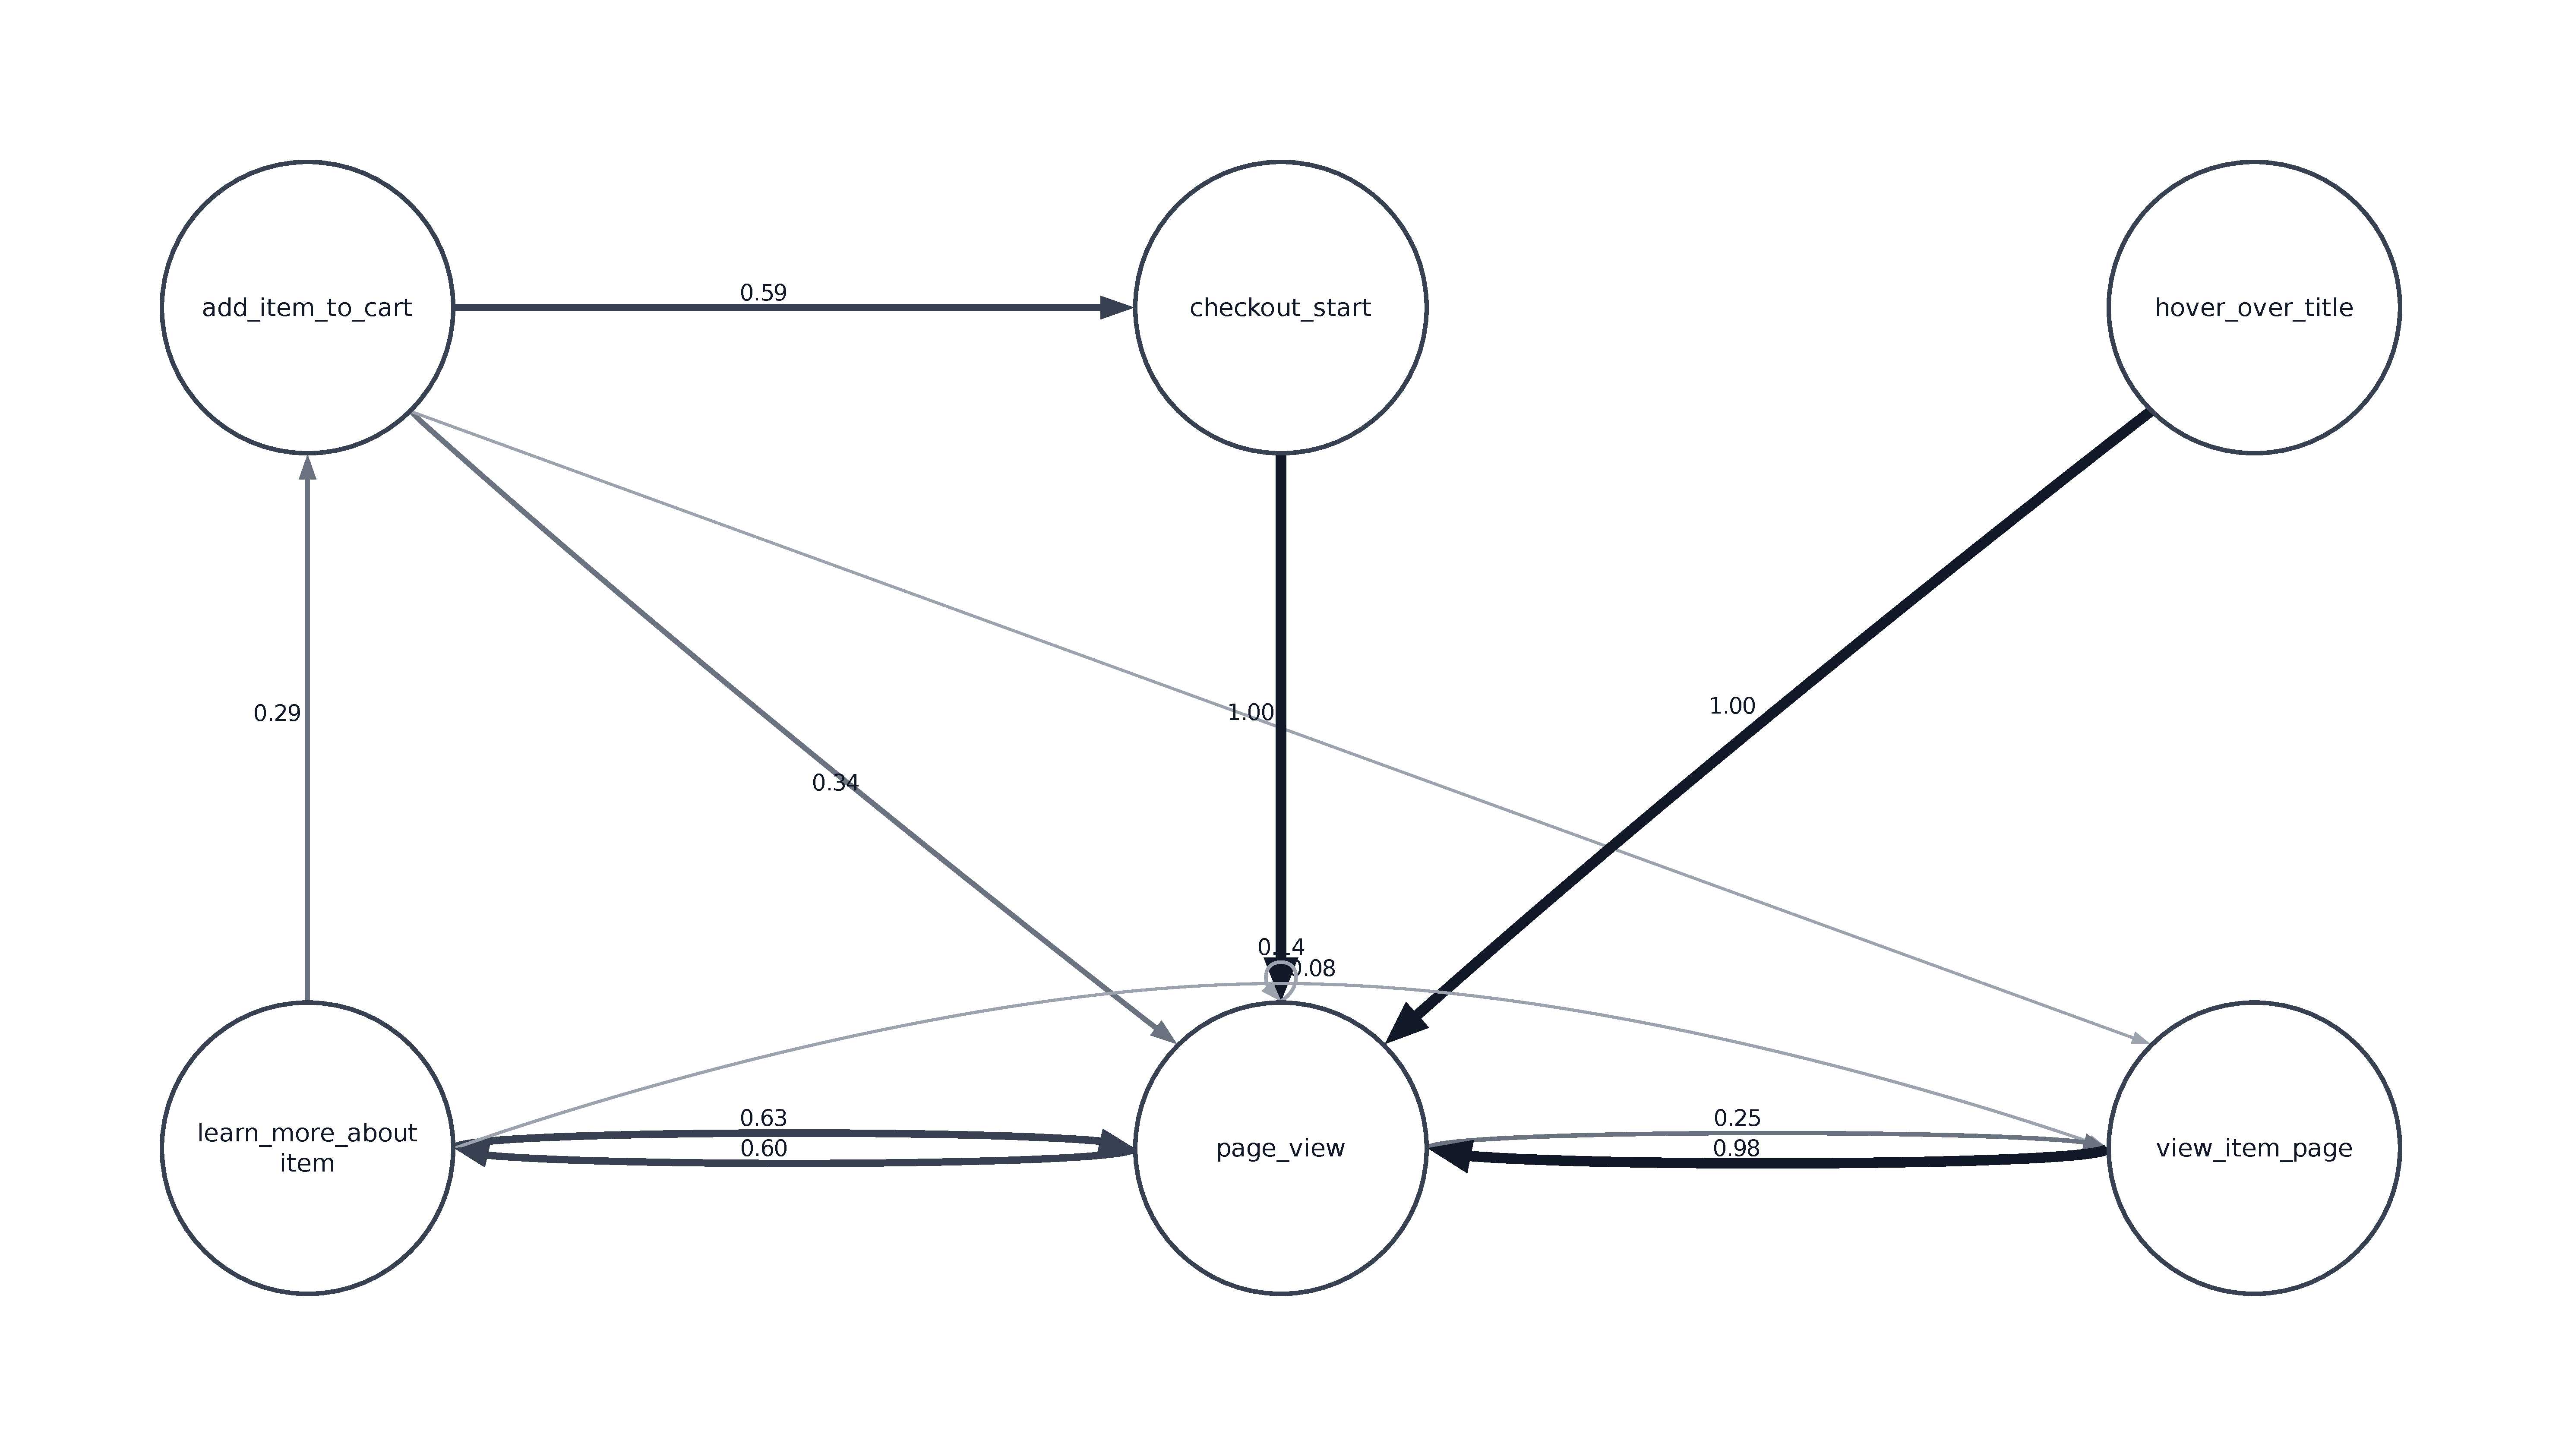
\includegraphics[width=0.75\linewidth,height=0.82\textheight,keepaspectratio]{mdp_agent.pdf}
\end{frame}

% ----- Threat model & evaluation -----

\begin{frame}{Appendix: threat model map}
  \centering
  \resizebox{0.98\linewidth}{!}{%
  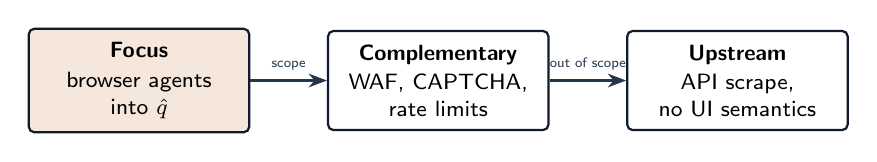
\begin{tikzpicture}[
    font=\sffamily\footnotesize,
    box/.style={draw=PhantomInk,rounded corners=2pt,thick,align=center,inner sep=5pt,minimum width=2.8cm},
    arr/.style={-Stealth,thick,PhantomSlate}
  ]
    \node[box,fill=PhantomCyan!18] (A) at (0,0) {\textbf{Focus}\\[0.15em]browser agents\\into \(\hat{q}\)};
    \node[box,fill=white] (B) at (3.8,0) {\textbf{Complementary}\\[0.15em]WAF, CAPTCHA,\\rate limits};
    \node[box,fill=white] (C) at (7.6,0) {\textbf{Upstream}\\[0.15em]API scrape,\\no UI semantics};
    \draw[arr] (A) -- node[above] {\tiny scope} (B);
    \draw[arr] (B) -- node[above] {\tiny out of scope} (C);
  \end{tikzpicture}%
  }
  \vfill
  \begin{block}{Claim boundary}
    Residual contamination after security controls is the motivating scenario.
  \end{block}
\end{frame}

\begin{frame}{Appendix: evaluation checklist (robustness culture)}
  \footnotesize
  \begin{enumerate}
    \item Session-aware labels: avoid splitting rows inside a trajectory if that inflates scores.
    \item Document how prototypes \(\bar{T}_H,\bar{T}_A\) were fit (full cohort vs.\ held-out); state explicitly in writing.
    \item Report temperature \(T\) as calibration, not as a tuned hyperparameter unless a sweep is shown.
    \item Separate \textbf{architecture} claims from \textbf{coverage} claims (hotel vs.\ airline balance at release).
  \end{enumerate}
\end{frame}

\begin{frame}{Appendix: sim-to-real gap (explicit)}
  \begin{itemize}
    \item Kernels and generators reflect a \textbf{small labeled cohort} and a \textbf{browser-use style} agent class.
    \item RL policies are trained in a \textbf{surrogate} market with engineered rewards and discretized prices.
    \item Deployment would require legal review, fairness testing, and refreshed baselines at scale.
  \end{itemize}
\end{frame}

\begin{frame}{Appendix: leakage surrogate (query-tax form)}
  \small
  \[
    \mathrm{COI}_{\mathrm{leak}}(p,\tau') \approx f(\tau')\cdot c_{\mathrm{info}}
  \]
  \begin{block}{Reading}
    \(f(\tau')\) is the weak agent score; \(c_{\mathrm{info}}\) is a minimal constant leakage proxy to expose the control channel. Revelation-style \(-\log \pi(p\mid\tau')\) is the natural upgrade.
  \end{block}
\end{frame}

\begin{frame}{Appendix: robust pricing template (symbolic)}
  \footnotesize
  \[
    \max_\pi\ \min_{Q\in\mathcal{U}_\epsilon(\hat{P}_N)} \mathbb{E}_{d\sim Q}\bigl[ R(p,d) - \lambda\,\mathrm{COI}_{\mathrm{leak}} - \eta\,\mathrm{UX} \bigr]
  \]
  \begin{alertblock}{Code-level substitute}
    Inner min over a \textbf{finite grid} of \(\alpha_k\in[\alpha_0\pm\epsilon_\alpha]\) around the nominal generator mix, not a continuous adversary over all \(Q\) in the ball.
  \end{alertblock}
\end{frame}

\begin{frame}{Appendix: Stackelberg timing (words)}
  \begin{itemize}
    \item Leader: platform sets price vector given current state and policy.
    \item Follower: demand proxy updates from simulated trajectories drawn from \(\mathcal{G}(\alpha)\) and kernels \((\hat{T}_H,\hat{T}_A)\).
    \item \textbf{Limbo} buffer stores alternating moves for a clean game history; relaxing strict alternation is listed future work.
  \end{itemize}
\end{frame}

\begin{frame}{Appendix: three layers of evidence}
  \footnotesize
  \begin{description}
    \item[Theorem 1] Formal COI erosion under independence and fixed-offer assumptions.
    \item[Simulator] Dynamic, adaptive pricing and contamination sweeps (different status).
    \item[Implementation] Local-$\alpha$ robust training; spirit of DRO without claiming a full numerical Wasserstein solver.
  \end{description}
\end{frame}

\begin{frame}{Appendix: composite strip (five plots, small multiples)}
  \centering
  {\footnotesize\itshape Same PDFs as the main talk, shrunk to scan the full panel at once.\par}
  \vspace{0.25em}
  \begin{columns}[T,onlytextwidth]
    \column{0.19\textwidth}
    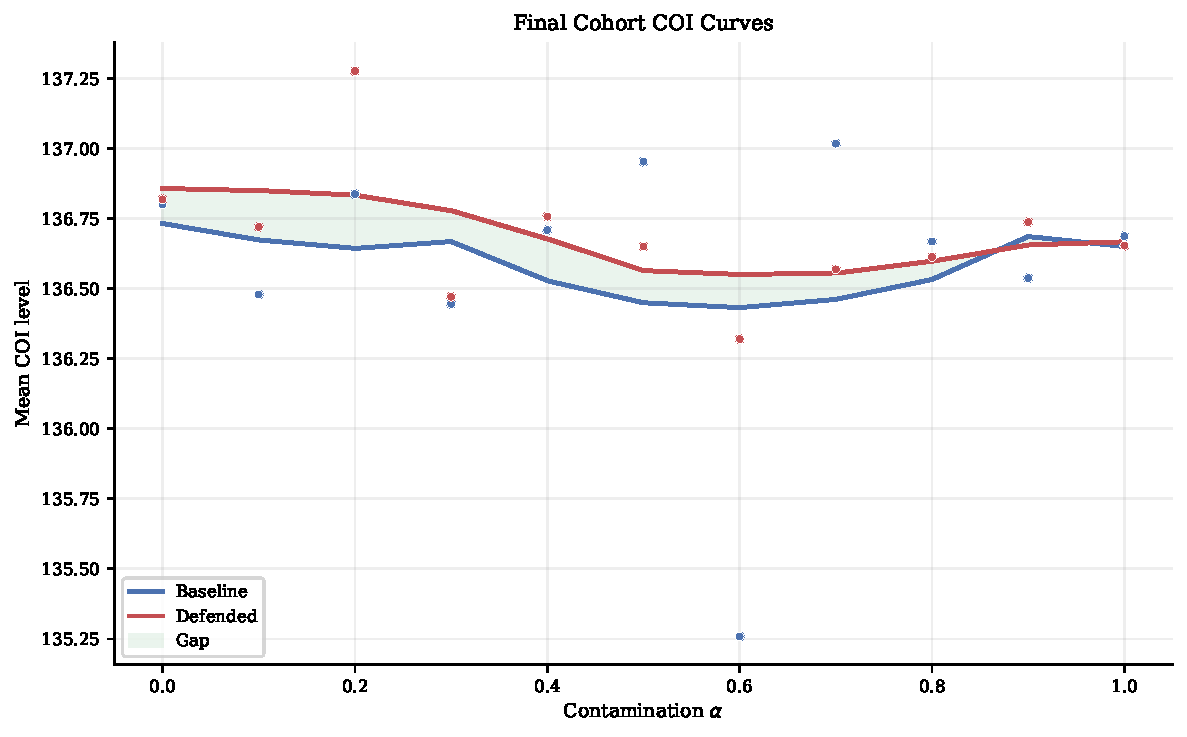
\includegraphics[width=\linewidth,height=0.26\textheight,keepaspectratio]{final_focus_coi_by_alpha.pdf}
    \column{0.19\textwidth}
    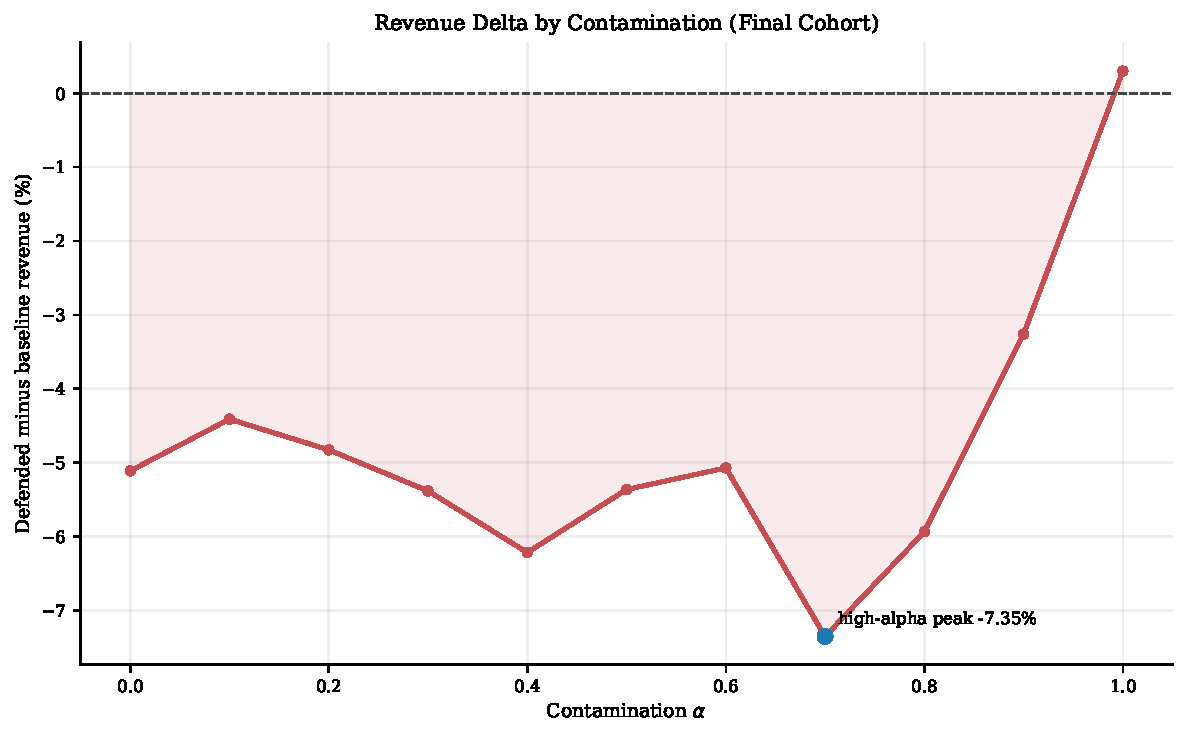
\includegraphics[width=\linewidth,height=0.26\textheight,keepaspectratio]{final_focus_revenue_delta.pdf}
    \column{0.19\textwidth}
    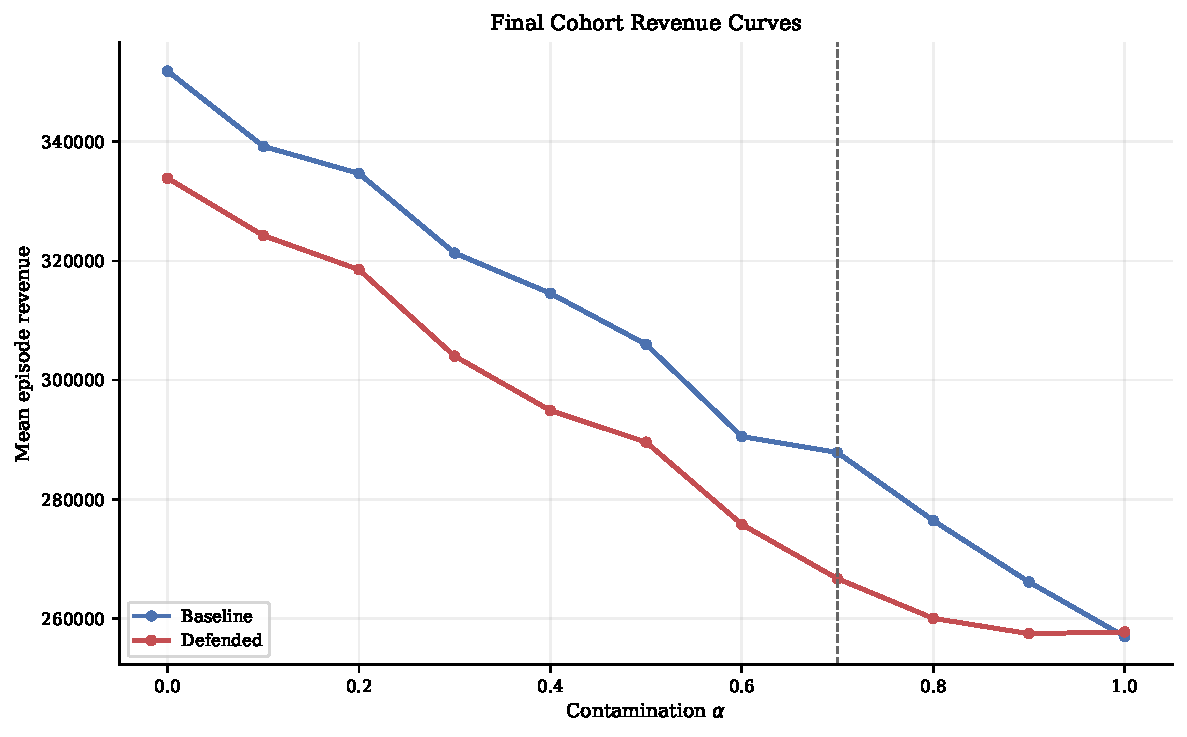
\includegraphics[width=\linewidth,height=0.26\textheight,keepaspectratio]{final_focus_revenue_by_alpha.pdf}
    \column{0.19\textwidth}
    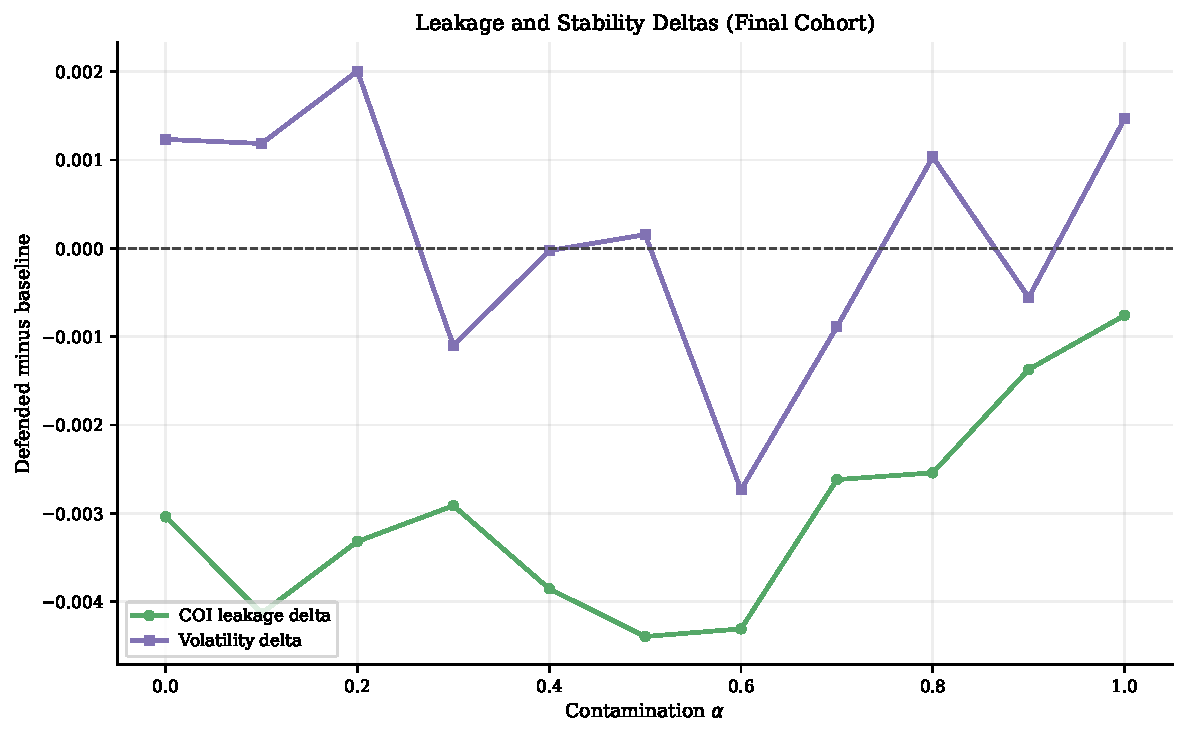
\includegraphics[width=\linewidth,height=0.26\textheight,keepaspectratio]{final_focus_risk_deltas.pdf}
    \column{0.19\textwidth}
    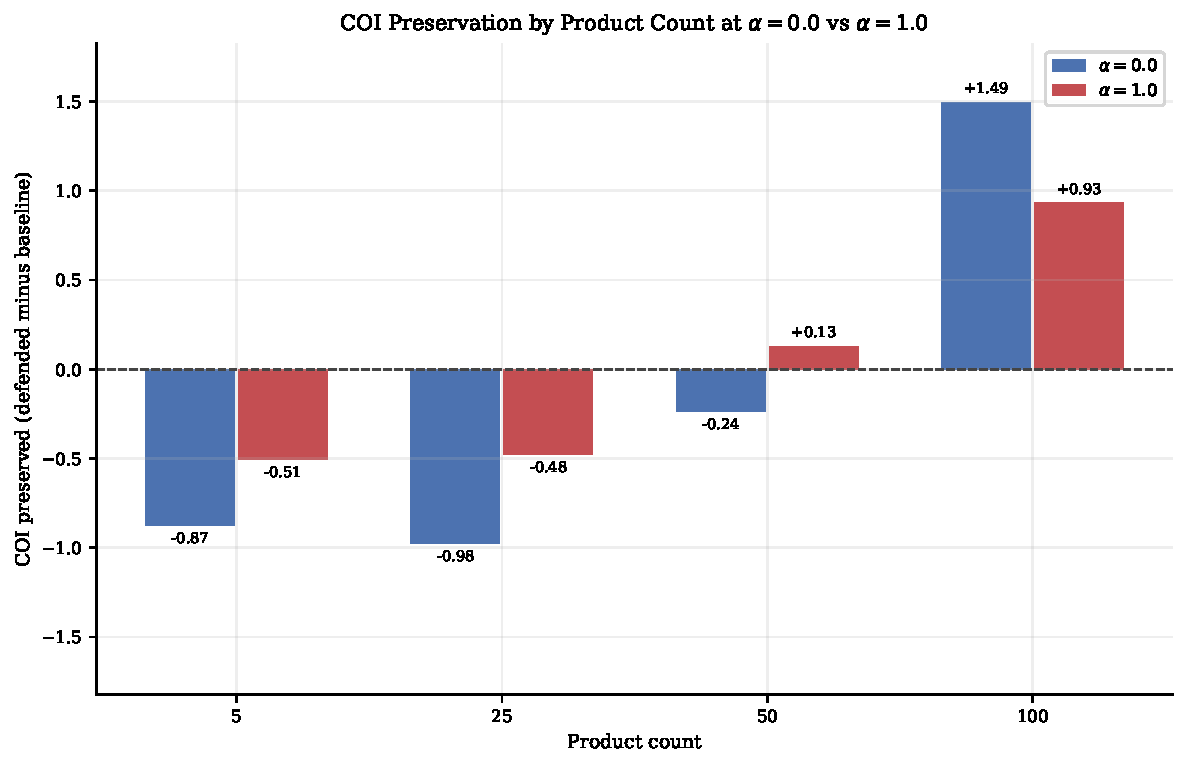
\includegraphics[width=\linewidth,height=0.26\textheight,keepaspectratio]{final_focus_coi_preservation_grid.pdf}
  \end{columns}
\end{frame}


\end{document}
